\chapter{PENGUJIAN DAN ANALISIS}
\vspace{4ex}

\hspace{\parindent} Pada bab ini menguraikan hasil pengujian serta analisa dari pengujian terhadap sistem yang telah dirancang pada Tugas Akhir ini. Pengujian ini dilakukan untuk menguji kemampuan sistem yang telah dibuat dalam menjawab permasalahan yang diangkat. Pengujian dibagi menjadi 2 bagian utama antara lain :
\begin{enumerate}[nolistsep]
	\item Pengujian Kebutuhan Sistem
	\item Pengujian Sistem oleh Pengguna
\end{enumerate}

Dengan dilaksanakannya serangkaian pengujian tersebut, sehingga dapat diambil kesimpulan terhadap penelitian Tugas Akhir ini. Dalam mengukur kemampuan sistem, \textit{completion rate} digunakan untuk mengukur banyaknya tugas yang berhasil dilakukan. Berdasarkan parameter tersebut, keberhasilan tugas bernilai 1 dan kegagalan bernilai 0. \textit{Completion rate} dapat dituliskan melalui persamaan \ref{eqn:completion_rate}. Semakin besar presentasenya, maka semakin efektif sistem tersebut dapat bekerja. 
\begin{equation}
	CompletionRate = \frac{Completed  \ task}{Total  \ of\   tasks} \cdot 100\%
	\label{eqn:completion_rate}
\end{equation}

Selain \textit{completion rate}, pengujian ini juga menggunakan \textit{likert scale} dalam pengukurannya yang berfungsi untuk menghitung rata-rata tingkat persetujuan terhadap suatu pernyataan yang dipilih. Berdasarkan parameter tersebut, nilainya tergantung dari opsi persetujuan yang digunakan. \textit{Agreement result} dari \textit{likert scale} dapat dituliskan melalui persamaan \ref{eqn:agreement_result} dengan $i$ adalah opsi tingkat persetujuan berdasarkan setiap pernyataan. Hasil akhirnya ditunjukkan sebagai perwakilan tingkat persetujuan dari pernyataan yang dianalisis.
\begin{equation}
	AgreementResult = \frac{\Sigma Total  \ of\   selected\ i \cdot Score[i]}{Total  \ of\   participats}
	\label{eqn:agreement_result}
\end{equation}
\vspace{2ex}

\section{Pengujian Kebutuhan Sistem}
\vspace{1ex}
	Pengujian sistem dilakukan untuk megevaluasi sistem secara keseluruhan berdasarkan spesifikasi dan kebutuhan yang menentukan kualitas sistem tersebut\cite{luo2001software}. Pengujian ini berkaitan dengan kemampuan sistem untuk menjalankan tugasnya dan mencapai tujuan sesuai dengan yang direncanakan. Secara umum, kebutuhan sistem dibagi menjadi 2 jenis yaitu kebutuhan fungsionalitas dan non fungsionalitas. Pengujian fungsionalitas adalah pengujian terhadap faktor internal yang membangun fitur atau layanan suatu sistem. Hal ini berkaitan dengan bagaimana sistem merespons suatu inputan. Sedangkan pengujian non fungsionalitas adalah pengujian terhadap faktor eksternal yang dapat memengaruhi fungsionalitas suatu sistem.\cite{sawant2012software}
\vspace{1.5ex}
	
	\subsection{Pengujian Penyajian Objek Hologram} 
	\vspace{1ex}
		Pengujian ini berkaitan dengan kebutuhan fungsionalitas sistem mengenai efek hologram manakah yang cocok diterapkan pada objek 3D yang akan diproyeksikan pada \textit{pyramid hologram}. Objek 3D yang diuji ditunjukkan pada gambar \ref{fig:objek3d}. 
		
		Skenario yang dilakukan yaitu saat berada di \textit{Main Scene} berupa menampilkan setiap objek 3D dalam efek hologram yang berbeda kemudian diproyeksikan dengan \textit{pyramid hologram}. Objek 3D hologram yang ditampilkan dinilai menggunakan sebuah opsi yang sesuai bedasarkan tingkat ketegasan objek dengan pilihan opsi :
		\begin{enumerate} [nolistsep]
			\item Sangat Baik (SB), yaitu objek sangat terlihat dengan jelas termasuk detailnya. 
			\item Baik (B), yaitu wujud objek masih terlihat meskipun detailnya tidak tajam.
			\item Kurang Baik (KB), yaitu objek terlihat tidak jelas (samar-samar).
		\end{enumerate}
	
		Banyaknya efek hologram yang digunakan dicontohkan pada gambar \ref{fig:sb_p1} dimana terdiri dari 4 perlakuan yang berbeda. Pemilihan efek hologram ini didasari dari 2 aspek, yaitu aspek  objek yang ditampilkan memiliki ilusi seperti benda padat atau cahaya hologram dan aspek warna objeknya seperti warna benda asli atau warna hologram. Menurut aspek pertama, gambar \ref{fig:ilusi1} dan \ref{fig:ilusi2} menampilkan objek seperti benda padat sedangkan gambar \ref{fig:ilusi3} dan \ref{fig:ilusi4} menampilkan objek selayaknya cahaya hologram yang terlihat semi-transparan serta memiliki efek \textit{glitch}. Jika menurut aspek kedua, gambar \ref{fig:ilusi1} dan \ref{fig:ilusi3} menampilkan objek dalam warna benda aslinya sedangkan gambar \ref{fig:ilusi2} dan \ref{fig:ilusi4} menampilkan objek dalam warna identik hologram berupa \textit{tosca} (semi biru-hijau). Dengan perlakuan di atas akan menentukan perlakuan manakah yang paling cocok untuk objek hologram, apakah sesuai dengan benda aslinya (benda padat dan warna asli) atau sesuai dengan ilusi khas hologram yang seharusnya (cahaya transparan dan warna \textit{tosca}) atau kombinasi keduanya.
		
		\vspace{-2ex}
		\begin{figure} [H]
			\subfloat[Efek Hologram A.\label{fig:ilusi1}]{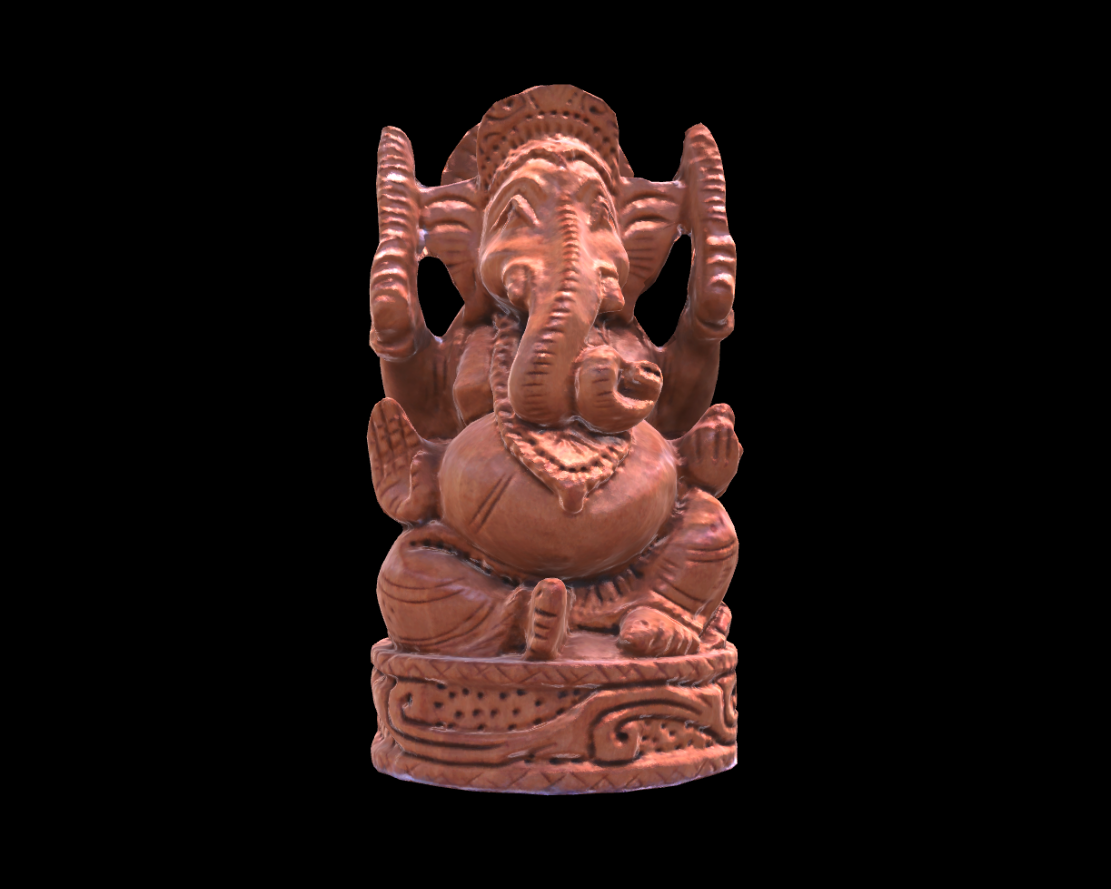
\includegraphics[width=0.4\textwidth]{img/bab4/ilusi1.png}}
			\hspace{4em}
			\subfloat[Efek Hologram B.\label{fig:ilusi2}]{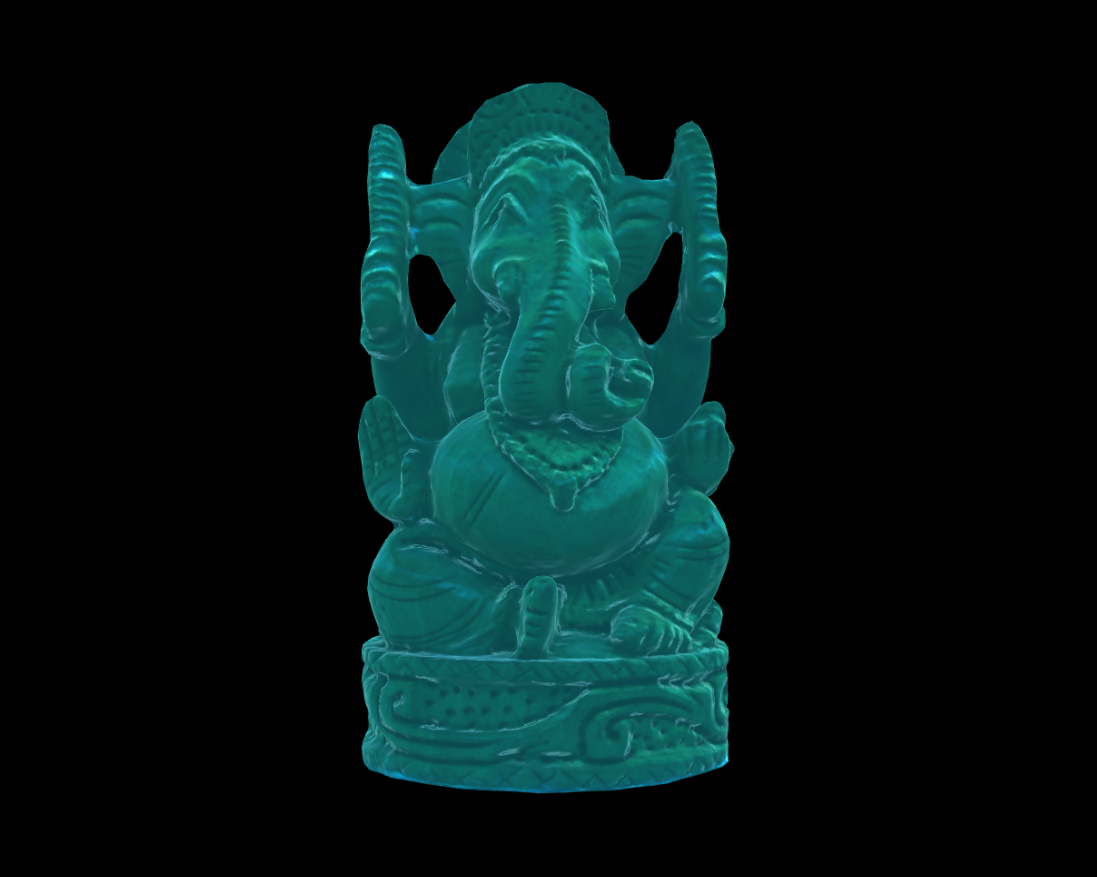
\includegraphics[width=0.4\textwidth]{img/bab4/ilusi2.png}}
			\\
			\subfloat[Efek Hologram C.\label{fig:ilusi3}]{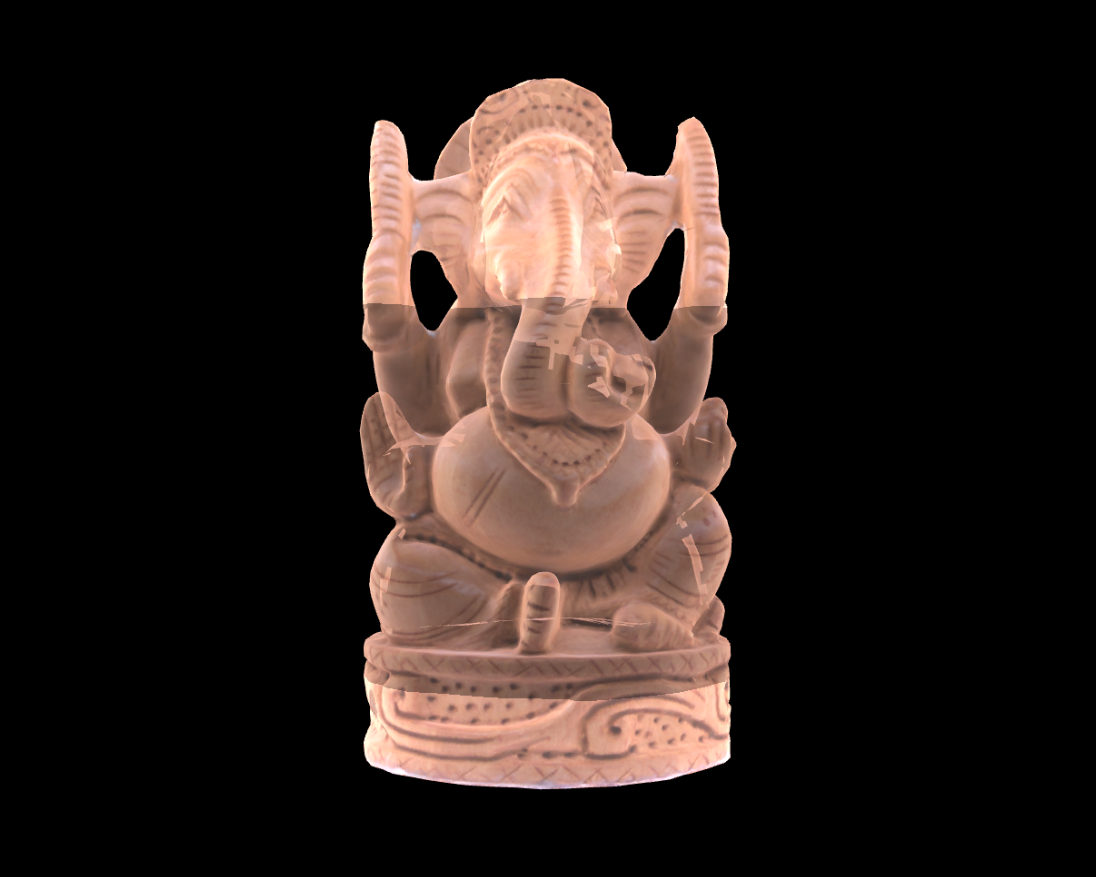
\includegraphics[width=0.4\textwidth]{img/bab4/ilusi3.png}}
			\hspace{4em}
			\subfloat[Efek Hologram D.\label{fig:ilusi4}]{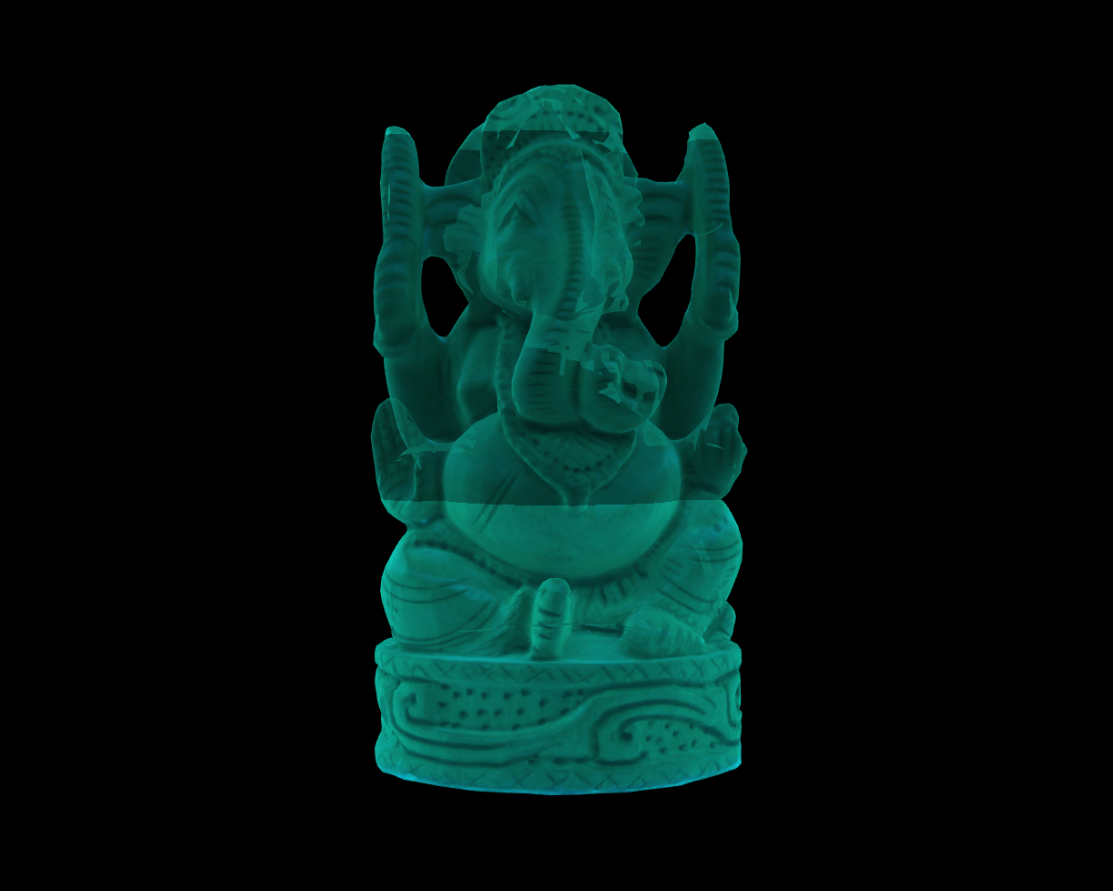
\includegraphics[width=0.4\textwidth]{img/bab4/ilusi4.png}}
			\caption{Efek hologram yang digunakan pada pengujian penyajian objek hologram.}
			\label{fig:sb_p1}
		\end{figure}
		\vspace{-2ex}
		
		Keempat efek hologram tersebut didapatkan dengan mengatur material objek yang bersesuaian, sehingga setiap objek memiliki nilai yang berbeda. Pada gambar \ref{fig:ilusi1} dan \ref{fig:ilusi2}, material objek diatur menggunakan material \textit{standard specular setup} untuk mengatur parameter yang berhubungan dengan permukaan objek seperti pemasangan \textit{texture map}. Sedangkan gambar \ref{fig:ilusi1} dan \ref{fig:ilusi3}, material objek diatur menggunakan \textit{shader} SFHologram untuk mengatur efek hologram seperti \textit{brigthness}, \textit{oppacity} dan \textit{glitch}\cite{hologramshader}.
		
		Pengukuran tingkat ketegasan objek dihitung dari banyaknya presentase total poin yang didapatkan dari total maksimal poin untuk setiap pernyataan yang disediakan (\textit{likert scale}). Berdasarkan parameter tersebut, setiap opsi memiliki poin yang berbeda yaitu SB=3 poin, B=2 poin, KB=1 poin. Semakin besar presentasenya, maka semakin tegas objek hologram dapat ditampilkan. Hasil pengujian dicantumkan melalui tabel \ref{tab:hasil_penyajian}.
		\vspace{-2ex}
		\begin{table}[H]
			\caption{Hasil pengujian penyajian hologram.}
			\label{tab:hasil_penyajian}
			\begin{tabular}{|C{0.4cm}|L{2.8cm}|C{1cm}|C{1cm}|C{1cm}|C{1cm}|}
				\hline
				\multirow{2}{*}{\textbf{No}} & \multicolumn{1}{c|}{\multirow{2}{*}{\textbf{Objek}}} & \multicolumn{4}{c|}{\textbf{Efek Hologram (poin)}} \\ \cline{3-6}
				& \multicolumn{1}{c|}{}& \multicolumn{1}{c|}{\textbf{A}} & \multicolumn{1}{c|}{\textbf{B}} & \multicolumn{1}{c|}{\textbf{C}} & \multicolumn{1}{c|}{\textbf{D}} \\ \hline
				1.&\textit{Hand Axe}		& 3 & 1 & 2 & 1 \\ \hline
				2.&\textit{Primeval Axe}	& 2 & 1 & 3 & 1 \\ \hline
				3.&\textit{Buddha Statue}	& 2 & 1 & 3 & 2 \\ \hline
				4.&\textit{Ganesha Statue}	& 2 & 1 & 3 & 3 \\ \hline
				5.&\textit{Brass Lamp}		& 2 & 1 & 3 & 2 \\ \hline
				6.&\textit{Ceramic Pot}		& 3 & 1 & 3 & 1 \\ \hline
				7.&\textit{Typewriter}		& 3 & 1 & 3 & 1 \\ \hline
				8.&\textit{Gramophone}		& 2 & 1 & 2 & 1 \\ \hline
				\multicolumn{2}{|c|}{\textbf{Total}} & 19 & 8 & 22 & 12 \\ \hline
				\multicolumn{2}{|c|}{\textit{\textbf{Effectivity}}} & 79.16\% & 10.00\% & 91.67\% & 45.83\% \\ \hline
			\end{tabular}
		\end{table}
		\vspace{-2ex}
		
		Pada efek hologram A yang menyerupai benda asli (benda pejal dan warna asli), tingkat ketegasan objek yang ditampilkan sebesar 79.16\% atau bernilai 19 dari 24 poin. Meskipun detail objek dapat ditampilkan lebih baik menyerupai model aslinya, namun tidak semua objek dengan efek ini memberikan tingkat visualisasi yang baik. Salah satu faktornya yaitu efek benda pejal memberikan ilusi seakan-akan objek tersebut hanya memiliki panjang dan lebar (dua dimensi). Hal ini disebabkan karena setiap sisi piramida hanya menampilkan proyeksi sisi tersebut tanpa adanya perpotongan pada sisi-sisi yang bertabrakan (warna objeknya padat).
		
		Efek hologram C berupa kombinasi dari cahaya semi - transparan layaknya hologram dengan warna asli benda dan memiliki efek \textit{glitch} memiliki tingkat efektivitas tertinggi sebesar 91.67\% atau bernilai 22 dari 24 poin. Dikarenakan objek yang dipantulkan memiliki karakteristik berupa semi-transparan, maka objek yang diproyeksikan pada perpotongan sisi piramida dapat terlihat dan menimbulkan ilusi membentuk objek tiga dimensi.
		
		Sedangkan efek hologram B dan D nilai efektivitasnya tidak terlalu tinggi dan objek yang ditampilkan pun tidak maksimal. Pada efek hologram B berupa benda pejal bernilai 10.00\% dimana bentuk objek terlihat sebagai benda dua dimensi. Pada efek hologram D berupa cahaya semi-transparan bernilai 45.83\% dimana cahaya semi-transparan dapat menampilkan ilusi benda tiga dimensi yang lebih baik daripada efek B. Kekurangan dari efek B dan D adalah penggunaan warna \textit{tosca} justru mengurangi kedetailan objek tersebut jika dibandingkan dengan warna aslinya.
		
		Dari hasil pengujian penyajian objek hologram didapatkan efek hologram dengan tingkat efektivitas tertinggi senilai 91.67\% pada efek hologram C, yaitu kombinasi dari warna asli objek yang dapat memperlihatkan detail yang lebih baik dan cahaya semi-transparan yang memperlihatkan panjang, tinggi, dan lebar sebagai objek tiga dimensi yang bervolume.	
	\vspace{1.5ex}
	
	\subsection{Pengujian Deteksi Pengindera Tangan} 
	\vspace{1ex}
		Pada penelitian ini, pengujian deteksi pengindera tangan berkaitan dengan kebutuhan fungsionalitas sistem sebagai inputan dari pengguna terhadap objek hologram. Pengujian ini mengenai kemampuan sistem untuk mengenali gestur tangan mengaktifkan responsnya. Melalui pengujian ini, performansi pengindera tangan juga dapat diukur dengan memperhitungkan kemampuan baca bervariasi gestur tangan.
		
		Variasi tangan ditunjukkan pada gambar \ref{fig:gestur_interaksi}. Skenario yang dilakukan yaitu melakukan interaksi dengan gestur tangan saat berada di \textit{Main Scene}. Setiap interaksi yang mengaktifkan respons dilakukan sebanyak 10 iterasi. Pengujian dihitung berdasarkan banyaknya respons yang berhasil diaktifkan berdasarkan fitur yang dibangun, baik dengan tangan kanan, kiri, maupun keduanya. Setiap skenario memiliki spesifikasi gestur dari tangan manakah yang dapat mengaktifkan respons tersebut. Hasil pengujian dicantumkan melalui tabel \ref{tab:hasil_deteksi}.
		
		Gestur tangan \textit{punch} atau genggaman seperti pada gambar \ref{fig:gs1a} dan \ref{fig:gs1b} digunakan untuk mengeksplorasi objek hologram berupa perputaran dan perpindahan di dalam \textit{workspace} yang telah ditentukan. Respons ini aktif jika hanya terdapat satu gestur genggaman yang terdeteksi, baik menggunakan tangan kanan ataupun tangan kiri. Sehingga pengujian hanya dilakukan pada tangan kanan dan tangan kiri secara terpisah.
		
		Gestur tangan \textit{pinch} atau cubitan seperti pada gambar \ref{fig:gs2} digunakan untuk memperbesar dan memperkecil objek hologram sebesar nilai yang telah ditentukan. Respons aktif hanya aktif jika kedua tangan kanan dan kiri membentuk gestur \textit{pinch} secara bersamaan dan diarahkan saling menjauh atau mendekat. Respons perbesaran aktif ketika kedua grstur saling berjauhan (ditarik keluar) dan sebaliknya menghasilkan pengecilan objek. Sehingga pengujian ini hanya dilakukan pada kedua tangan sekaligus untuk 2 skenario pebesaran dan pengecilan yang berbeda.
		
		Gestur tangan \textit{gun} atau tembakan seperti pada gambar \ref{fig:gs3a}, \ref{fig:gs3b}, dan \ref{fig:gs3c}  digunakan untuk mengaktifkan animasi objek \textit{primeval axe}. Respons ini dapat aktif jika seminimal mungkin terdapat satu tangan yang membentuk gestur \textit{gun}artinya animasi dapat diputar dengan banyak kondisi (tangan kanan, tangan kiri, atau keduanya). Untuk mengetahui tangan manakah yang paling efektif untuk mengaktifkan animasi, maka pengujian dilakukan pada tangan kanan, tangan kiri, maupun keduanya secara bersamaan.
		
		Gestur tangan \textit{high five} seperti pada gambar \ref{fig:gs4} digunakan untuk mengembalikan objek ke posisi, rotasi, dan ukuran awal. Respons ini hanya aktif jika kedua tangan kanan dan kiri membentuk gestur \textit{high five} secara bersamaan, sehingga pengujian terpisah antara tangan kanan dan kiri tidak dilakukan.
		
		Gestur tangan \textit{side thumb} seperti pada gambar \ref{fig:gs5a} dan \ref{fig:gs5b} digunakan untuk mengganti objek dan informasi yang ditampilkan. Respons ini dapat aktif secara efektif jika hanya terdapat salah satu tangan yang dideteksi karena pergantian objeknya berbeda. Gestur \textit{side thumb} pada tangan kanan akan menampilkan objek setelahnya, sedangkan pada tangan kiri akan menampilkan objek sebelumnya. 
		
		Gestur tangan \textit{upside} seperti pada gambar \ref{fig:gs6} digunakan untuk menampilkan menu \textit{Help} saat \textit{Main Scene} dijalankan. Sedangkan gestur tangan \textit{home} seperti pada gambar \ref{fig:gs7} digunakan untuk menampilkan \textit{Main Menu} atau keluar dari \textit{Main Scene} yang sedang berjalan. Respons yang bersesuaian dari kedua gestur ini hanya aktif jika kedua tangan kanan dan kiri membentuk gestur secara bersamaan, sehingga pengujian dilakukan pada kedua tangan.
		
		\vspace{-2ex}
		\begin{table}[H]
			\caption{Hasil pengujian deteksi pengindera tangan.}
			\label{tab:hasil_deteksi}
			\begin{tabular}{|C{0.4cm}|m{2.9cm}|C{1cm}|C{1cm}|C{1cm}|C{1cm}|}
				\hline
				\multirow{2}{*}{\textbf{No}} & \multirow{2}{*}{\parbox{2.8cm}{\centering \textbf{Interaksi dan Pola Tangan}}} & \multicolumn{3}{c|}{{\parbox{3cm}{\textbf{Tangan yang Digunakan (iterasi)}}}}&\multicolumn{1}{c|}{\multirow{2}{*}{\textbf{Total}}} \\ \cline{3-5}
				&& \textbf{Kiri} & \textbf{Kanan} & \textbf{Kedua} & \multicolumn{1}{c|}{}\\ \hline
				1.& Mengeksplorasi objek 							& 10 & 10 & -  & 20 \\ \hline
				2.& Memperbesar objek (\textit{zoom in}) 			& -  & -  & 10 & 10	\\ \hline
				3.& Memperkecil objek (\textit{zoom out}) 			& -  & -  & 10 & 10	\\ \hline
				4.& Mengaktifkan animasi objek						& 9  & 9  & 10 & 28	\\ \hline
				5.& Mengembalikan objek (\textit{reset to default} 	& -  & -  & 9  & 9	\\ \hline
				6.& Menampilkan objek sebelumnya					& 10 & -  & -  & 10 \\ \hline
				7.& Menampilkan objek setelahnya					& -  & 10 & -  & 10	\\ \hline
				8.& Membuka tampilan \textit{ Help}						& -  & -  & 8  & 8	\\ \hline
				9.& Membuka tampilan \textit{Go To Main Menu}						& -  & -  & 8  & 8	\\ \hline
				10.& Membatalkan pilihan (\textit{back} atau \textit{cancel})			& 4  & 3  & -  & 7	\\ \hline
				11.& Menyetujui pilihan (OK)						& 3  & 4  & -  & 7	\\ \hline				
				\multicolumn{2}{|c|}{\textbf{Total}}&36&36&55&127 \\ \hline
				\multicolumn{2}{|c|}{\textit{\textbf{Completion Rate}}}&72.00\%&72.00\%&97.50\% & 90.71\%\\ \hline
			\end{tabular}
		\end{table}
		\vspace{-2ex}
		
		Gestur tangan \textit{thumb down} seperti pada gambar \ref{fig:gs8a} dan \ref{fig:gs8b} dan gestur tangan \textit{thumb down} seperti pada gambar \ref{fig:gs8c} dan \ref{fig:gs8d} digunakan untuk memilih suatu opsi yang ditampilkan. Respons ini dapat aktif jika salah satu tangan yang dideteksi karena pilihannya yang berbeda. Gestur \textit{thumb down} berfungsi membatalkan pilihan layaknya opsi \textit{back} dan \textit{cancel}, sedangkan gestur \textit{thumb up} berfungsi untuk menyetujui pilihan layaknya opsi OK. 
		
		Pada gestur untuk mengaktifkan eksplorasi objek (rotasi dan posisi), baik tangan kiri ataupun tangan kanan, dapat dilakukan sebanyak 10 kali dari 10 iterasi. Kondisi ini juga terjadi pada gestur untuk mengaktifkan \textit{zoom in}, \textit{zoom out}, dan mengganti objek sebelum dan sesudahnya.
		
		Pada gestur untuk mengaktifkan animasi objek, respons yang bersesuaian hanya muncul 9 kali dari 10 iterasi baik pada tangan kiri ataupun tangan kanan. Hal ini disebabkan gestur tangan \textit{gun} yang menekuk \textit{ring} dan \textit{pinky fingers} seperti pada penelitian ini terkadang terdeteksi memanjang (tidak menutup), sehingga detektor tidak mengembalikan nilai \textit{true} pada \textit{Extended Finger Detector}. Untuk meminimalisir kondisi ini, gestur aktivasi animasi juga dibuat bisa aktif jika terdapat kedua tangan kanan dan kiri secara bersamaan dimana terbukti dengan keberhasilan 10 kali dari 10 iterasi saat gestur dilakukan pada kedua tangan.
		
		Kondisi ketidak stabilan gestur yang terdeteksi juga ditemukan pada gestur yang mengaktifkan \textit{reset to default} dimana berhasil memicu respons 9 kali dari 10 iterasi. Hal ini disebabkan detektor harus membaca secara tepat arah \textit{index finger} sebesar y=1, sehingga meskipun semua jari sudah terbuka menghadap ke depan (mengarah ke objek) tetapi arah \textit{index finger} tidak tepat menghadap sumbu yang bersesuaian maka respons tidak muncul.
		
		Pengenalan gestur yang tidak stabil sering ditemukan pada pada gestur untuk mengaktifkan pergantian menu yang bersesuaian. Untuk gestur yang membuka menu \textit{Help} berupa \textit{upside} dapat memicu respons yang sesuai sebanyak 8 kali dari 10 iterasi yang diakibatkan terkadang detektor mendeteksi telapak tangan menghadap ke atas (sumbu y=1). Pada gestur yang membuka \textit{Main Menu} berupa \textit{home} juga memiliki nilai keberhasilan yang sama, yaitu 8 kali dari 10 iterasi, jika posisi \textit{index finger} tidak sesuai maka respons yang dipicu adalah \textit{reset} objek dimana kedua gestur ini memiliki pola yang hampir sama.
		
		Ketidak stabilan tertinggi muncul papda gestur untuk membatalkan dan menyetujui pilihan yang bersesuaian. Gestur \textit{thumb down} untuk  membatalkan pilihan pada tangan kiri memicu respons sebanyak 4 dari 10 iterasi dan tangan kanan sebesar 3 dari 10 iterasi, hal ini diakibatkan detektor harus membaca secara tepat posisi \textit{thumb index} pada arah y=-1. Sedangkan pada gestur \textit{thumb up} untuk menyetujui pilihan dengan tangan kiri memicu respons sebanyak 3 dari 10 iterasi dan tangan kanan sebesar 4 dari 10 iterasi, hal ini disebabkan \textit{thumb index} terkadang tertutup oleh \textit{finger index} yang lain dikarenakan posisi Leap Motion Controller yang berada tepat di bawah tangan pengguna.
		
		Dari hasil pengujian deteksi pengindera tangan dengan total iterasi sebanyak 160 iterasi, didapatkan nilai sebesar 90.71\% gestur dapat dikenali oleh sistem dimana 72.00\% interaksi dapat dipicu oleh masing-masing tangan kiri dan tangan kanan serta sebesar 97.50\% keberhasilan oleh kedua tangan secara bersamaan (kanan dan kiri).
	\vspace{1.5ex}	
	
	\subsection{Pengujian Performansi Sistem} 
	\label{section:p3}
	\vspace{1ex}
		Performansi adalah salah satu kebutuhan non fungsionalitas sistem untuk mengetahui kemampuan kinerja sistem secara keseluruhan. Pada penelitian ini, sistem akan diuji pada tiga buah \textit{server computer} dengan spesifikasi yang berbeda seperti ditunjukkan pada \ref{tab:spesifikasi_pc}. Perbedaan ini memengaruhi daya komputasi yang dimiliki masing-masing komputer, sehingga memberikan dampak pada performansi sistem yang diuji. Hal ini dilakukan untuk mengetahui \textit{minimum requirement} yang dibutuhkan agar sistem dapat bekerja. 
	
		Pengujian ini disebut sebagai \textit{benchmark}, yaitu pengukuran dan evaluasi kemampuan suatu perangkat menggunakan nilai standard yang telah ditentukan. Nilai standard atau skenario yang digunakan yaitu saat berada di \textit{Main Scene} berupa mengeksplorasi masing-masing objek hologram yang ditampilkan, memutar objek, mengganti objek yang ditampilkan, dan menjalankan animasi. Pengujian dilakukan sebanyak 5 kali iterasi pada tiap \textit{server computer} dengan skenario yang sama. Parameter yang digunakan dalam menganalisis pengujian ini adalah kondisi \textit{frame rate} pada setiap \textit{server}\cite{graphy}.
		
				\vspace{-2ex}
		\begin{table}[H]
			\caption{Spesifikasi \textit{server computer} untuk pengujian performansi.}
			\label{tab:spesifikasi_pc}
			\begin{tabular}{|C{1.6cm}|C{2.2cm}|C{2.5cm}|C{2.17cm}|}
				\hline
				\textbf{Spesifikasi}  & \textbf{PC 1} 					& \textbf{PC 2}				& \textbf{PC 3} \\ \hline
				Nama Produk           & Asus ROG Strix G351GT			& Asus ROG Strix GL553VD	& Notebook Asus X450CP   \\ \hline
				\textit{Processor}    & Intel Core i7-9750H 			& Intel Core i7-7700HQ		& Intel Core i3-3217U     \\ \hline
				\textit{Graphic Card} & NVIDIA GeForce GTX 1650   		& NVIDIA GeForce GTX 1050	& AMD Radeon R5 M240    \\ \hline
				\textit{Storage Unit} & 512 GB SSD            			& 1TB HDD + 128 GB SSD		& 500 GB HDD     \\ \hline
				RAM                   & 16 GB							& 16 GB              		& 10 GB     \\ \hline
				Sistem Operasi        &	Windows 10 Home Edition 64-bit	& Windows 10 Education 64-bit & Windows 10 Pro 64-bit               \\ \hline
			\end{tabular}
		\end{table}
		
		\subsubsection{Pengujian Performansi pada PC 1}
		\vspace{1ex}
			\vspace{-2ex}
			\begin{table}[H]
				\caption{Hasil pengujian performansi pada \textit{server computer} 1.}
				\label{tab:p3_pc1}
				\begin{tabular}{|c|c|c|c|}
					\hline
					\multirow{2}{*}{\textbf{Iterasi}} & \multicolumn{3}{c|}{\textit{\textbf{Frame Rate}}\textbf{ (fps)}} \\ \cline{2-4} 
					& \textbf{Avg.}   & \textbf{Min.}  & \textbf{Max.}  \\ \hline
					1& 58.12 & 22.69 & 81.04 \\ \hline
					2& 55.81 & 24.65 & 76.98 \\ \hline
					3& 59.12 & 25.79 & 79.39 \\ \hline
					4& 54.84 & 24.64 & 81.64 \\ \hline
					5& 57.93 & 24.24 & 80.44 \\ \hline
				\end{tabular}
			\end{table}
			\vspace{-2ex}
		
			Hasil pengujian sesuai dengan skenario yang ditetapkan pada \textit{server computer} 1 ditunjukkan melalui tabel \ref{tab:p3_pc1}. \textit{Server computer} 1 merupakan \textit{server} dengan spesifikasi tertinggi pada penelitian ini. Berdasarkan grafik \ref{fig:p3_a}, perubahan \textit{frame rate} pada \textit{server computer} 1 terhitung cukup stabil dengan nilai rata-rata sebesar 57.16, nilai minimum sebesar 24.40, dan nilai maksimum sebesar 79.29. Selisih antara nilai minimum dan maksimum setiap iterasi pun terhitung kecil dan stabil. Perubahan terbesar terjadi pada awal (frame ke-4) sewaktu aplikasi dijalankan dikarenakan adanya peralihan \textit{game scene} ketika pengguna memasuki \textit{Main Scene} dan \textit{Main Menu}. Pada saat pengujian, perubahan \textit{frame} saat objek dieksplorasikan memperlihatkan pergerakan objek yang halus dan stabil.
	
			\vspace{-2ex}
			\begin{figure}[H]
				\begin{tikzpicture}
				\begin{axis}[
				grid=major,
				xlabel=\textbf{Frame},
				ylabel=\textbf{Frame Rate (fps)}]
				\addplot[color=blue] coordinates {
					(0,0)
					(1,42.89746)
					(2,0.8521035)
					(3,69.89048)
					(4,102.216)
					(5,52.89242)
					(6,54.54556)
					(7,66.20587)
					(8,58.46176)
					(9,44.94887)
					(10,61.72687)
					(11,78.98083)
					(12,63.34446)
					(13,57.79612)
					(14,61.18378)
					(15,61.8131)
					(16,56.80915)
					(17,62.57196)
					(18,57.45179)
					(19,54.63585)
					(20,60.83132)
					(21,63.21472)
					(22,60.35258)
					(23,56.75014)
					(24,56.84983)
					(25,62.81723)
					(26,39.43777)
					(27,35.0652)
					(28,42.19587)
					(29,50.37098)
					(30,42.34561)
					(31,58.66789)
					(32,57.48647)
					(33,49.89248)
					(34,49.54027)
					(35,57.57715)
					(36,57.32335)
					(37,73.19733)
					(38,57.82453)
					(39,59.87666)
					(40,65.86097)
					(41,58.94419)
					(42,60.36315)
					(43,56.07959)
					(44,61.29254)
					(45,64.32233)
					(46,62.33326)
					(47,54.49651)
					(48,64.1153)
					(49,59.84297)
					(50,47.57464)
					(51,57.25868)
					(52,61.61163)
					(53,56.76206)
					(54,59.66979)
					(55,58.91641)
					(56,47.99155)
					(57,60.17137)
					(58,62.67313)
					(59,63.68859)
					(60,36.62306)
					(61,59.53834)
					(62,52.35355)
					(63,57.12001)
					(64,63.22312)
					(65,62.00204)
					(66,64.75761)
					(67,60.11313)
					(68,59.29861)
					(69,59.97289)
					(70,48.42521)
					(71,46.1076)
					(72,62.80066)
					(73,59.18105)
					(74,55.2923)
					(75,65.36887)
					(76,59.75072)
					(77,53.31883)
					(78,60.00564)
					(79,38.9742)
					(80,44.70493)
					(81,59.01063)
					(82,61.30606)
					(83,53.25636)
					(84,76.76011)
					(85,57.95388)
					(86,40.65586)
					(87,68.31441)
					(88,63.4385)
					(89,61.9126)
					(90,52.01994)
					(91,62.939)
					(92,52.34808)
					(93,60.36205)
					(94,63.70076)
					(95,58.87513)
					(96,61.73792)
					(97,58.94766)
					(98,59.56387)
					(99,60.10483)
					(100,56.8948)
					(101,57.15494)
					(102,57.71673)
					(103,59.75822)
					(104,58.53259)
					(105,60.96817)
					(106,57.36182)
					(107,66.02708)
					(108,59.46965)
					(109,55.58057)
					(110,36.4113)
					(111,58.10102)
					(112,59.65021)
					(113,59.62176)
					(114,60.36752)
					(115,64.66841)
					(116,61.94827)
					(117,60.91358)
					(118,64.82814)
					(119,59.8104)
					(120,40.9831)
					(121,60.93066)
					(122,58.15881)
					(123,59.24522)
					(124,61.7162)
					(125,57.68842)
					(126,68.09531)
					(127,55.14625)
					(128,61.63443)
					(129,61.49116)
					(130,39.67593)
					(131,63.41717)
					(132,60.90653)
					(133,47.34893)
					(134,59.19121)
					(135,57.99421)
					(136,61.59721)
					(137,62.48946)
					(138,60.09074)
					(139,65.43817)
					(140,61.26363)
					(141,60.38538)
					(142,55.03789)
					(143,61.62227)
					(144,60.76441)
					(145,59.42229)
					(146,56.95961)
					(147,30.17429)
					(148,49.47629)
					(149,62.13264)
					(150,45.70426)
					(151,59.58375)
					(152,58.31482)
					(153,63.80888)
					(154,54.217)
					(155,63.49045)
					(156,61.67357)
					(157,59.55572)
					(158,61.54717)
					(159,61.67053)
					(160,48.59228)
					(161,63.74949)
					(162,60.09615)
					(163,60.92583)
					(164,60.69766)
					(165,60.8665)
					(166,63.90103)
					(167,62.43015)
					(168,60.86834)
					(169,45.56805)
					(170,74.38207)
					(171,62.59468)
					(172,50.02201)
					(173,55.97161)
					(174,60.34785)
					(175,62.90891)
					(176,66.80741)
					(177,61.46697)
					(178,47.52242)
					(179,59.46081)
					(180,46.89398)
					(181,60.04672)
					(182,54.68156)
					(183,71.06613)
					(184,60.36424)
					(185,62.34219)
					(186,59.159)
					(187,59.2196)
					(188,62.58684)
					(189,61.02063)
					(190,46.30016)
					(191,60.43136)
					(192,58.08179)
					(193,59.65662)
					(194,58.38223)
					(195,61.8433)
					(196,60.47814)
					(197,59.20417)
					(198,59.71646)
					(199,61.34179)
					(200,51.8726)
					(201,61.15909)
					(202,61.47189)
					(203,60.57229)
					(204,57.58246)
					(205,61.94521)
					(206,62.63702)
					(207,65.99483)
					(208,55.5056)
					(209,59.46399)
					(210,51.05662)
					(211,60.19998)
					(212,58.63383)
					(213,58.78273)
					(214,61.6386)
					(215,62.07209)
					(216,58.82215)
					(217,60.40508)
					(218,48.36034)
					(219,60.76626)
					(220,52.38701)
					(221,49.46479)
					(222,61.1733)
					(223,41.03456)
					(224,62.93029)
					(225,62.45667)
					(226,61.55929)
					(227,88.06073)
					(228,61.30306)
					(229,60.60826)
					(230,42.00445)
					(231,60.9652)
					(232,58.5439)
					(233,57.92971)
					(234,62.02204)
					(235,62.21575)
					(236,64.19927)
					(237,67.13798)
					(238,60.03194)
					(239,59.29088)
					(240,48.96608)
					(241,59.98153)
					(242,59.3074)
					(243,60.66158)
					(244,59.80682)
					(245,59.32606)
					(246,63.10223)
					(247,64.44088)
					(248,60.53085)
					(249,64.6542)
					(250,40.2251)
					(251,58.60256)
					(252,56.17851)
					(253,56.78269)
					(254,54.55984)
					(255,61.29254)
					(256,58.34578)
					(257,37.34074)
					(258,53.11238)
					(259,45.00328)
					(260,45.59132)
					(261,64.9064)
					(262,60.33875)
					(263,59.49548)
					(264,66.35832)
					(265,61.24486)
					(266,60.62553)
					(267,60.52133)
					(268,58.60703)
					(269,58.03157)
					(270,55.29506)
					(271,60.48802)
					(272,49.12556)
					(273,55.42408)
					(274,48.43788)
					(275,52.80835)
					(276,51.86803)
					(277,55.77743)
					(278,51.94886)
					(279,47.85651)
					(280,39.15289)
					(281,49.00591)
					(282,51.12213)
					(283,45.77266)
					(284,51.88121)
					(285,59.62425)
					(286,57.82821)
					(287,53.72531)
					(288,55.77556)
					(289,54.78792)
					(290,52.26545)
					(291,55.18246)
					(292,58.61631)
					(293,58.41292)
					(294,53.92231)
					(295,57.08609)
					(296,58.85261)
					(297,49.68993)
					(298,58.25299)
					(299,61.04335)
					(300,51.18886)
					(301,62.2084)
					(302,57.78042)
					(303,57.69375)
					(304,57.22068)
					(305,50.46708)
					(306,52.03888)
					(307,61.51499)
					(308,61.09556)
					(309,59.22417)
					(310,48.03904)
					(311,59.06744)
					(312,58.03864)
					(313,60.97821)
					(314,65.01613)
					(315,66.31651)
					(316,48.53615)
					(317,47.17538)
					(318,49.41346)
					(319,48.94355)
					(320,35.70205)
					(321,49.58891)
					(322,59.98188)
					(323,55.56821)
					(324,52.47416)
					(325,55.17393)
					(326,54.34842)
					(327,58.53465)
					(328,51.48668)
					(329,72.94744)
					(330,51.08609)
					(331,59.10061)
					(332,56.86859)
					(333,49.28706)
					(334,59.09257)
					(335,45.44463)
					(336,58.52608)
					(337,50.35424)
					(338,50.94736)
					(339,48.29425)
					(340,53.76893)
					(341,54.13071)
					(342,55.7961)
					(343,49.60785)
					(344,45.20898)
					(345,44.42253)
					(346,58.2323)
					(347,50.51832)
					(348,51.79791)
					(349,51.59799)
					(350,47.90465)
					(351,59.54295)
					(352,56.86665)
					(353,66.19141)
					(354,56.05256)
					(355,60.44488)
					(356,63.53603)
					(357,57.85832)
					(358,59.92222)
					(359,50.31523)
					(360,37.64777)
					(361,54.03361)
					(362,45.80139)
					(363,56.02555)
					(364,62.76242)
					(365,68.00177)
					(366,62.35736)
					(367,56.54925)
					(368,52.90054)
					(369,57.55561)
					(370,54.43332)
					(371,54.38152)
					(372,52.54695)
					(373,56.80302)
					(374,54.22905)
					(375,48.9098)
					(376,52.3404)
					(377,55.40749)
					(378,57.8038)
					(379,56.31709)
					(380,34.9223)
					(381,53.0918)
					(382,50.87971)
					(383,52.38894)
					(384,59.19051)
					(385,59.22767)
					(386,60.33364)
					(387,54.82666)
					(388,53.34927)
					(389,54.31801)
					(390,44.40497)
					(391,55.5093)
					(392,56.16242)
					(393,50.25909)
					(394,54.67708)
					(395,55.56358)
					(396,54.78822)
					(397,56.7141)
					(398,53.99422)
					(399,56.81108)
					(400,53.02311)
					(401,54.71777)
					(402,57.54899)
					(403,56.16494)
					(404,56.58733)
					(405,54.43391)
					(406,61.5957)
					(407,56.79785)
					(408,48.62607)
					(409,55.40105)
					(410,45.21756)
					(411,54.50839)
					(412,53.21952)
					(413,55.62756)
					(414,57.71073)
					(415,57.39803)
					(416,46.77246)
					(417,67.32103)
					(418,59.48875)
					(419,60.20071)
					(420,42.59542)
					(421,60.818)
					(422,62.90851)
					(423,63.94761)
					(424,59.90499)
					(425,65.24136)
					(426,56.82593)
					(427,57.98748)
					(428,60.09507)
					(429,64.15356)
					(430,45.07184)
					(431,57.55727)
					(432,59.03257)
					(433,47.63017)
					(434,52.94311)
					(435,51.97316)
					(436,47.47076)
					(437,53.39741)
					(438,70.09575)
					(439,62.10756)
					(440,40.98361)
					(441,65.71037)
					(442,57.82119)
					(443,58.52026)
					(444,58.77651)
					(445,61.78637)
					(446,51.58149)
					(447,54.212)
					(448,59.62318)
					(449,64.22691)
					(450,58.52471)
					(451,61.97208)
					(452,58.69544)
					(453,59.98225)
					(454,61.29367)
					(455,58.53773)
					(456,63.28233)
					(457,61.29554)
					(458,61.33239)
					(459,51.52382)
					(460,41.29348)
					(461,57.94716)
					(462,57.63556)
					(463,62.09869)
					(464,53.60263)
					(465,43.68548)
					(466,54.60363)
					(467,49.53143)
					(468,60.41128)
					(469,44.26502)
					(470,40.96514)
					(471,64.1223)
					(472,46.90783)
					(473,60.08315)
					(474,57.19352)
					(475,59.05105)
					(476,59.10724)
					(477,69.00026)
					(478,60.65017)
					(479,60.64134)
					(480,38.13839)
					(481,57.221)
					(482,58.17877)
					(483,57.59009)
					(484,58.85954)
					(485,64.17785)
					(486,61.74479)
					(487,60.22427)
					(488,55.62076)
					(489,66.61693)
					(490,50.12909)
					(491,61.50137)
					(492,59.45303)
					(493,56.73888)
					(494,62.34103)
					(495,63.7304)
					(496,53.6035)
					(497,58.02854)
					(498,59.38383)
					(499,59.08559)
					(500,41.74668)
					(501,61.14039)
					(502,57.90824)
					(503,62.09444)
					(504,55.59756)
					(505,60.80913)
					(506,58.07842)
					(507,59.27296)
					(508,57.53773)
					(509,66.30421)
					(510,45.00916)
					(511,55.79517)
					(512,60.82836)
					(513,58.18995)
					(514,58.13244)
					(515,61.09855)
					(516,59.32536)
					(517,60.47009)
					(518,63.96029)
					(519,71.91606)
					(520,48.01344)
					(521,57.49737)
					(522,59.37431)
					(523,54.78732)
					(524,65.23115)
					(525,54.08387)
					(526,60.70171)
					(527,65.75919)
					(528,59.63065)
					(529,60.89875)
					(530,37.19878)
					(531,58.76097)
					(532,57.10794)
					(533,57.34109)
					(534,60.76664)
					(535,60.29508)
					(536,64.62788)
					(537,59.13206)
					(538,55.44866)
					(539,54.53663)
					(540,39.76601)
					(541,67.22961)
					(542,58.53567)
					(543,60.54992)
					(544,60.78695)
					(545,58.82803)
					(546,59.33908)
					(547,63.22712)
					(548,62.87489)
					(549,58.15543)
					(550,37.94764)
					(551,63.15963)
					(552,58.82872)
					(553,45.23904)
					(554,49.34958)
					(555,59.64701)
					(556,67.49506)
					(557,62.18983)
					(558,56.41399)
					(559,61.88655)
					(560,41.77493)
					(561,71.21645)
					(562,45.64022)
					(563,68.37513)
					(564,68.64596)
					(565,63.25591)
					(566,63.72714)
					(567,59.27999)
					(568,59.50468)
					(569,62.42821)
					(570,41.04888)
					(571,61.30117)
					(572,59.80289)
					(573,59.31198)
					(574,60.65532)
					(575,64.55319)
					(576,59.97649)
					(577,59.28315)
					(578,59.3796)
					(579,61.86396)
					(580,39.84556)
					(581,65.05208)
					(582,61.10303)
					(583,59.69365)
					(584,62.4247)
					(585,59.97685)
					(586,61.21787)
					(587,61.43525)
					(588,58.65206)
					(589,63.75884)
					(590,38.52867)
					(591,63.01833)
					(592,66.60716)
					(593,60.31072)
					(594,62.53713)
					(595,56.86374)
					(596,44.23115)
					(597,49.25308)
					(598,55.49605)
					(599,60.53856)
					(600,55.1575)
					(601,54.04675)
					(602,65.50848)
					(603,58.98731)
					(604,61.47302)
					(605,59.14256)
					(606,61.06647)
					(607,60.90987)
					(608,62.57901)
					(609,64.95826)
					(610,49.73714)
					(611,63.4969)
					(612,65.89482)
					(613,60.85761)
					(614,47.20053)
					(615,51.9432)
					(616,67.08573)
					(617,46.07191)
					(618,50.8541)
					(619,56.21672)
					(620,62.44224)
					(621,59.22627)
					(622,54.50453)
					(623,62.53948)
					(624,59.74894)
					(625,60.67961)
					(626,58.03392)
					(627,58.69096)
					(628,58.34068)
					(629,60.44305)
					(630,39.10787)
					(631,65.14488)
					(632,60.58844)
					(633,60.11674)
					(634,59.7236)
					(635,61.20176)
					(636,63.12055)
					(637,59.38383)
					(638,65.21455)
					(639,61.45299)
					(640,48.78525)
					(641,51.09549)
					(642,52.27309)
					(643,41.4924)
					(644,76.34928)
					(645,58.66789)
					(646,62.13303)
					(647,56.81366)
					(648,63.44855)
					(649,51.65049)
					(650,41.14803)
					(651,87.27298)
					(652,60.51474)
					(653,65.99223)
					(654,57.03075)
					(655,57.64719)
					(656,47.43316)
					(657,64.31199)
					(658,59.85192)
					(659,63.90389)
					(660,40.08257)
					(661,64.87103)
					(662,57.78443)
					(663,55.70286)
					(664,58.01945)
					(665,54.3068)
					(666,54.82125)
					(667,87.85107)
					(668,59.61714)
					(669,60.10483)
					(670,44.73392)
					(671,64.90894)
					(672,56.18419)
					(673,57.05841)
					(674,60.3606)
					(675,59.36339)
					(676,61.11312)
					(677,57.15037)
					(678,57.08512)
					(679,58.77686)
					(680,41.81284)
					(681,57.96564)
					(682,55.1715)
					(683,58.80451)
					(684,73.8727)
					(685,58.69854)
					(686,63.2491)
					(687,58.60291)
					(688,53.79381)
					(689,66.63024)
					(690,39.51788)
					(691,60.16703)
					(692,61.60595)
					(693,54.34369)
					(694,57.56655)
					(695,61.67434)
					(696,62.24441)
					(697,60.43611)
					(698,44.94947)
					(699,61.26475)
					(700,36.44846)
					(701,53.47021)
					(702,62.68177)
					(703,63.53684)
					(704,61.86435)
					(705,61.06535)
					(706,59.06151)
					(707,61.95057)
					(708,59.47424)
					(709,55.05425)
					(710,54.64332)
					(711,63.28793)
					(712,64.50822)
					(713,60.48875)
					(714,65.10798)
					(715,68.10133)
					(716,60.8058)
					(717,55.976)
					(718,69.05743)
					(719,64.53236)
					(720,43.05371)
					(721,50.68295)
					(722,50.71302)
					(723,53.6147)
					(724,53.59057)
					(725,60.23153)
					(726,58.19164)
					(727,58.92822)
					(728,58.7475)
					(729,74.25117)
					(730,40.79651)
					(731,44.87666)
					(732,46.15037)
					(733,53.16349)
					(734,56.4054)
					(735,59.1786)
					(736,60.07882)
					(737,62.98102)
					(738,55.89903)
					(739,57.59838)
					(740,56.87473)
					(741,59.43431)
					(742,62.41145)
					(743,59.01028)
					(744,59.85121)
					(745,58.75303)
					(746,55.22025)
					(747,61.3305)
					(748,62.67785)
					(749,64.1898)
					(750,56.44965)
					(751,58.55144)
					(752,62.66017)
					(753,59.86697)
					(754,58.77893)
					(755,60.65311)
					(756,59.84011)
					(757,55.64458)
					(758,56.01927)
					(759,57.58909)
					(760,38.26287)
					(761,77.09982)
					(762,59.63029)
					(763,61.45942)
					(764,60.5877)
					(765,53.76951)
					(766,61.07616)
					(767,47.78698)
					(768,55.69107)
					(769,60.93697)
					(770,37.84109)
					(771,58.5703)
					(772,63.41757)
					(773,61.21674)
					(774,56.35644)
					(775,58.62387)
					(776,53.3103)
					(777,55.56667)
					(778,49.44767)
					(779,66.96309)
					(780,45.05661)
					(781,59.1604)
					(782,56.18767)
					(783,56.50579)
					(784,59.11528)
					(785,62.40094)
					(786,59.04024)
					(787,63.49166)
					(788,59.405)
					(789,59.34612)
					(790,37.60006)
					(791,63.01793)
					(792,58.58952)
					(793,63.13091)
					(794,61.81845)
					(795,57.17193)
					(796,56.92881)
					(797,55.4459)
					(798,58.15509)
					(799,52.60666)
					(800,41.41301)
					(801,56.86859)
					(802,61.62227)
					(803,58.85989)
					(804,64.10831)
					(805,63.09467)
					(806,60.95108)
					(807,58.67099)
					(808,63.98444)
					(809,54.72046)
					(810,40.46453)
					(811,58.4744)
					(812,57.29313)
					(813,51.26917)
					(814,56.70381)
					(815,81.76214)
					(816,59.75393)
					(817,59.97145)
					(818,52.92209)
					(819,49.57563)
					(820,37.30104)
					(821,60.85094)
					(822,61.42091)
					(823,61.70173)
					(824,59.7393)
					(825,67.85503)
					(826,59.35141)
					(827,63.43367)
					(828,59.32641)
					(829,60.85353)
					(830,36.55679)
					(831,54.51611)
					(832,53.44507)
					(833,53.41367)
					(834,62.51915)
					(835,61.06385)
					(836,51.00584)
					(837,73.07965)
					(838,58.71267)
					(839,46.55342)
					(840,35.26528)
					(841,56.9301)
					(842,63.76087)
					(843,63.79585)
					(844,59.1429)
					(845,55.14047)
					(846,55.83847)
					(847,65.54153)
					(848,50.7066)
					(849,46.44229)
					(850,39.20062)
					(851,63.00999)
					(852,60.30308)
					(853,64.93675)
					(854,53.50913)
					(855,51.56952)
					(856,46.68142)
					(857,60.04564)
					(858,60.52462)
					(859,46.76809)
					(860,33.46194)
					(861,62.5794)
					(862,51.81321)
					(863,55.95094)
					(864,51.21167)
					(865,51.8605)
					(866,56.94534)
					(867,55.42838)
					(868,64.73917)
					(869,59.09013)
					(870,45.08363)
					(871,75.21115)
					(872,49.06049)
					(873,58.19773)
					(874,54.66393)
					(875,56.48888)
					(876,63.689)
					(877,57.30232)
					(878,52.29168)
					(879,63.54411)
					(880,42.50924)
					(881,56.74789)
					(882,52.28703)
					(883,56.07393)
					(884,53.2436)
					(885,55.15051)
					(886,53.09688)
					(887,61.13217)
					(888,72.20216)
					(889,47.99432)
					(890,49.68648)
					(891,64.45791)
					(892,69.60492)
					(893,55.69386)
					(894,57.0132)
					(895,64.0615)
					(896,88.6077)
					(897,56.8576)
					(898,59.30811)
					(899,66.07246)
					(900,39.27745)
					(901,62.82828)
					(902,62.90891)
					(903,59.97829)
					(904,66.82661)
					(905,62.72817)
					(906,60.6476)
					(907,55.52286)
					(908,55.30148)
					(909,48.29448)
					(910,47.58392)
					(911,47.92347)
					(912,59.82543)
					(913,53.87002)
					(914,59.80325)
					(915,64.46082)
					(916,63.81458)
					(917,60.45986)
					(918,60.0132)
					(919,65.18693)
					(920,57.97976)
					(921,62.63035)
					(922,57.54303)
					(923,61.30795)
					(924,61.15796)
					(925,68.88713)
					(926,60.97226)
					(927,67.34188)
					(928,50.72537)
					(929,49.39882)
					(930,41.48052)
					(931,39.72858)
					(932,41.91589)
					(933,53.72474)
					(934,57.18174)
					(935,54.91337)
					(936,57.1024)
					(937,50.87635)
					(938,56.67263)
					(939,56.71635)
					(940,51.78771)
					(941,42.13915)
					(942,48.44328)
					(943,58.68958)
					(944,56.83401)
					(945,56.51985)
					(946,62.14384)
					(947,62.0956)
					(948,58.41394)
					(949,61.42657)
					(950,53.25948)
					(951,57.41451)
					(952,59.62851)
					(953,61.93523)
					(954,54.30946)
					(955,66.668)
					(956,59.27929)
					(957,60.94737)
					(958,57.64819)
					(959,62.66528)
					(960,42.60831)
					(961,54.04237)
					(962,57.373)
					(963,57.1605)
					(964,59.86984)
					(965,52.67871)
					(966,58.91745)
					(967,52.34177)
					(968,55.04365)
					(969,50.77637)
					(970,63.39666)
					(971,63.41717)
					(972,40.8809)
					(973,48.07461)
					(974,42.01945)
					(975,43.84734)
					(976,54.07364)
					(977,51.54852)
					(978,49.8885)
					(979,61.43487)
					(980,49.31039)
					(981,53.21895)
					(982,54.58485)
					(983,58.59536)
					(984,49.38003)
					(985,60.30417)
					(986,50.10748)
					(987,54.56609)
					(988,55.47666)
					(989,54.17911)
					(990,35.17387)
					(991,57.20987)
					(992,49.59579)
					(993,56.88218)
					(994,62.43561)
					(995,63.21392)
					(996,58.67959)
					(997,57.47589)
					(998,59.61251)
					(999,54.62243)
					(1000,51.35896)
					(1001,51.87583)
					(1002,57.73405)
					(1003,57.43957)
					(1004,53.68724)
					(1005,56.93042)
					(1006,59.36515)
					(1007,55.02366)
					(1008,56.37265)
					(1009,57.32269)
					(1010,58.38359)
					(1011,50.99959)
					(1012,59.27752)
					(1013,55.32442)
					(1014,50.95749)
					(1015,56.92005)
					(1016,57.7644)
					(1017,62.20375)
					(1018,56.08902)
					(1019,55.19921)
					(1020,46.89816)
					(1021,52.15368)
					(1022,54.19966)
					(1023,47.96094)
					(1024,64.65963)
					(1025,61.68803)
					(1026,56.92783)
					(1027,49.888)
					(1028,46.10356)
					(1029,49.40833)
					(1030,39.59549)
					(1031,56.24835)
					(1032,58.02315)
					(1033,73.91803)
					(1034,55.51423)
					(1035,48.19208)
					(1036,50.37276)
					(1037,57.39573)
					(1038,48.47921)
					(1039,57.0314)
					(1040,40.44522)
					(1041,62.07441)
					(1042,60.33364)
					(1043,58.6352)
					(1044,60.69287)
					(1045,58.92717)
					(1046,62.96952)
					(1047,65.99832)
					(1048,64.13792)
					(1049,62.79001)
					(1050,64.32233)
					(1051,51.59107)
					(1052,56.47388)
					(1053,60.37991)
					(1054,58.96957)
					(1055,60.88614)
					(1056,57.01807)
					(1057,54.59797)
					(1058,58.86404)
					(1059,54.41584)
					(1060,34.95905)
					(1061,53.1344)
					(1062,53.35866)
					(1063,56.8043)
					(1064,55.63313)
					(1065,54.60691)
					(1066,52.34698)
					(1067,55.07791)
					(1068,56.8576)
					(1069,53.81668)
					(1070,38.48981)
					(1071,64.57738)
					(1072,61.68993)
					(1073,66.70535)
					(1074,60.67078)
					(1075,57.76707)
					(1076,57.87707)
					(1077,55.43237)
					(1078,62.59624)
					(1079,60.94514)
					(1080,42.78935)
					(1081,53.53119)
					(1082,58.81384)
					(1083,49.10771)
					(1084,54.48878)
					(1085,60.14929)
					(1086,59.67406)
					(1087,56.30789)
					(1088,64.95995)
					(1089,61.88463)
					(1090,39.60098)
					(1091,70.612)
					(1092,55.1983)
					(1093,56.37296)
					(1094,48.27536)
					(1095,54.8977)
					(1096,81.09708)
					(1097,57.06916)
					(1098,49.39906)
					(1099,46.405)
					(1100,47.6356)
					(1101,70.20451)
					(1102,59.47956)
					(1103,55.7103)
					(1104,53.67283)
					(1105,57.50894)
					(1106,60.98454)
					(1107,59.33204)
					(1108,61.67281)
					(1109,54.75222)
					(1110,38.4116)
					(1111,58.03426)
					(1112,56.82819)
					(1113,76.26543)
					(1114,56.07928)
					(1115,66.56859)
					(1116,59.93227)
					(1117,57.54137)
					(1118,55.81479)
					(1119,61.04224)
					(1120,57.37169)
					(1121,67.63338)
					(1122,56.63637)
					(1123,62.5841)
					(1124,60.07305)
					(1125,61.99128)
					(1126,62.40016)
					(1127,69.16634)
					(1128,59.11004)
					(1129,56.60078)
					(1130,43.20289)
					(1131,54.32775)
					(1132,59.00819)
					(1133,55.8391)
					(1134,56.39045)
					(1135,68.27197)
					(1136,61.98398)
					(1137,60.90876)
					(1138,59.68546)
					(1139,62.26262)
					(1140,40.83033)
					(1141,59.79252)
					(1142,59.88132)
					(1143,57.54501)
					(1144,61.85249)
					(1145,61.94597)
					(1146,65.01824)
					(1147,58.63246)
					(1148,69.8446)
					(1149,61.27901)
					(1150,47.29049)
					(1151,58.43921)
					(1152,58.29408)
					(1153,61.67814)
					(1154,64.50156)
					(1155,59.16739)
					(1156,54.42295)
					(1157,62.02666)
					(1158,49.3031)
					(1159,48.69355)
					(1160,52.88487)
					(1161,59.64665)
					(1162,45.44174)
					(1163,52.50998)
					(1164,51.9432)
					(1165,67.09428)
					(1166,55.18581)
					(1167,51.5743)
					(1168,48.82765)
					(1169,47.38528)
					(1170,37.20114)
					(1171,47.55971)
					(1172,50.21038)
					(1173,54.119)
					(1174,53.57392)
					(1175,52.25343)
					(1176,41.51169)
					(1177,45.71094)
					(1178,63.16481)
					(1179,57.61563)
					(1180,40.53326)
					(1181,59.21154)
					(1182,59.74858)
					(1183,57.87372)
					(1184,58.22484)
					(1185,58.32468)
					(1186,62.10601)
					(1187,56.61007)
					(1188,52.21687)
					(1189,60.10085)
					(1190,41.91906)
					(1191,61.37379)
					(1192,56.80398)
					(1193,54.98433)
					(1194,60.92657)
					(1195,59.8659)
					(1196,63.85044)
					(1197,60.13483)
					(1198,71.22152)
					(1199,56.76175)
					(1200,50.22425)
					(1201,60.96371)
					(1202,58.64312)
					(1203,58.50245)
					(1204,60.37517)
					(1205,62.30335)
					(1206,60.81282)
					(1207,61.36023)
					(1208,62.61153)
					(1209,63.0688)
					(1210,45.17099)
					(1211,61.32825)
					(1212,59.77966)
					(1213,60.57742)
					(1214,59.13835)
					(1215,60.90504)
					(1216,60.27764)
					(1217,62.98339)
					(1218,83.09512)
					(1219,62.27386)
					(1220,40.86854)
					(1221,62.89388)
					(1222,59.71896)
					(1223,62.36786)
					(1224,58.03392)
					(1225,57.0015)
					(1226,63.77755)
					(1227,70.04272)
					(1228,63.01833)
					(1229,63.46064)
					(1230,41.73013)
					(1231,58.1605)
					(1232,61.48776)
					(1233,61.82571)
					(1234,61.78293)
					(1235,62.43522)
					(1236,60.83206)
					(1237,64.11037)
					(1238,61.66445)
					(1239,67.13978)
					(1240,58.64518)
					(1241,62.88319)
					(1242,63.29394)
					(1243,61.76881)
					(1244,64.13628)
					(1245,62.49219)
					(1246,59.39618)
					(1247,62.43951)
					(1248,64.36415)
					(1249,57.95321)
					(1250,43.95025)
					(1251,57.65982)
					(1252,66.04322)
					(1253,56.14476)
					(1254,63.81458)
					(1255,55.63932)
					(1256,61.18566)
					(1257,67.59086)
					(1258,59.68617)
					(1259,66.72093)
					(1260,43.7019)
					(1261,73.11545)
					(1262,70.94714)
					(1263,58.95809)
					(1264,44.48973)
					(1265,58.57853)
					(1266,54.18292)
					(1267,62.9604)
					(1268,61.96363)
				};
				\end{axis}
				\node[above,font=\bfseries] at (current bounding box.north) {Server Computer 1};
				\node[red, pin={[pin distance=3.5cm]12:{%
						\begin{tikzpicture}
						\begin{axis}[
						grid=major,
						every axis plot post/.append style={thick},
						tiny,
						xmin=3,xmax=5,
						ymin=100,ymax=105,
						]
						\addplot[color=blue] coordinates {
							(3,69.89048)
							(4,102.216)
							(5,52.89242)};
						\end{axis}
						\end{tikzpicture}%
				}},draw,rectangle,minimum size=0.5cm] at (0.5 , 5.2) {};
				\end{tikzpicture}
				\caption{Grafik \textit{frame rate} pada \textit{server computer} 1.} 
				\label{fig:p3_a}
			\end{figure}
			
		\subsubsection{Pengujian Performansi pada PC 2}
			\vspace{1ex}
			Hasil pengujian sesuai dengan skenario yang ditetapkan pada \textit{server computer} 2 ditunjukkan melalui tabel \ref{tab:p3_pc2}. \textit{Server computer} 2 merupakan \textit{server} utama yang digunakan dalam pembuatan sistem \textit{interactive holographic projection}. Di antara ketiga \textit{server computer} yang digunakan, PC 2 memiliki spesifikasi yang tidak jauh berbeda dengan PC 1. Hasil pengujian antara keduanya pun tidak jauh berbeda, secara umum pun pergerakan objek ketika dieksplorasikan terlihat cukup stabil meskipun tidak sebaik pada PC 1. Berdasarkan grafik \ref{fig:p3_b}, perubahan \textit{frame rate} pada \textit{server computer} 2 ini memiliki nilai  rata-rata 57.30, nilai minimum sebesar 25.26, serta nilai maksimum sebesar 90.38. Beberapa lonjakan \textit{frame rate} terjadi saat ada perubahan suatu gestur interaksi, seperti objek yang berhenti setelah aktivasi animasi objek selesai diputar.
			
			\vspace{-2ex}
			\begin{table}[H]
				\caption{Hasil pengujian performansi pada \textit{server computer} 2.}
				\label{tab:p3_pc2}
				\begin{tabular}{|c|c|c|c|}
					\hline
					\multirow{2}{*}{\textbf{Iterasi}} & \multicolumn{3}{c|}{\textit{\textbf{Frame Rate}}\textbf{ (fps)}} \\ \cline{2-4} 
					& \textbf{Avg.}   & \textbf{Min.}  & \textbf{Max.}  \\ \hline
					1& 57.39 & 27.56 & 96.58 \\ \hline
					2& 57.87 & 30.48 & 88.19 \\ \hline
					3& 56.58 & 24.00 & 91.51 \\ \hline
					4& 57.57 & 21.64 & 88.89 \\ \hline
					5& 57.10 & 23.11 & 86.74 \\ \hline
				\end{tabular}
			\end{table}
			\vspace{-2ex}
			
			\vspace{-2ex}
			\begin{figure} [H]
				\begin{tikzpicture}
				\begin{axis}[
				grid=major,
				xlabel=\textbf{Frame},
				ylabel=\textbf{Frame Rate (fps)}]
				\addplot[color=blue] coordinates {
					(0,0)
					(1,25.08617)
					(2,0.6063611)
					(3,45.20203)
					(4,52.1227)
					(5,51.86587)
					(6,49.04894)
					(7,53.59574)
					(8,51.49118)
					(9,44.69374)
					(10,51.31073)
					(11,46.54193)
					(12,49.54444)
					(13,50.40501)
					(14,49.88253)
					(15,48.13988)
					(16,49.11977)
					(17,49.78716)
					(18,47.90557)
					(19,107.6878)
					(20,61.47604)
					(21,57.2554)
					(22,56.15233)
					(23,56.48122)
					(24,59.76608)
					(25,56.9515)
					(26,53.95693)
					(27,57.32138)
					(28,59.13661)
					(29,57.68743)
					(30,58.53156)
					(31,52.85691)
					(32,52.51549)
					(33,51.89414)
					(34,75.7329)
					(35,71.46788)
					(36,60.67667)
					(37,79.10641)
					(38,69.8168)
					(39,75.96879)
					(40,79.92519)
					(41,60.38465)
					(42,74.5601)
					(43,74.12953)
					(44,53.83319)
					(45,71.86231)
					(46,70.44189)
					(47,70.84109)
					(48,70.99651)
					(49,69.4348)
					(50,73.90164)
					(51,55.67432)
					(52,62.04398)
					(53,74.46571)
					(54,62.39977)
					(55,79.85626)
					(56,70.11197)
					(57,70.45876)
					(58,54.64302)
					(59,62.64761)
					(60,64.02705)
					(61,60.12542)
					(62,61.44091)
					(63,62.4099)
					(64,62.68924)
					(65,74.02143)
					(66,59.87235)
					(67,58.81419)
					(68,59.19787)
					(69,66.29937)
					(70,76.14175)
					(71,61.7711)
					(72,59.76144)
					(73,66.70046)
					(74,64.47411)
					(75,67.69839)
					(76,68.0499)
					(77,68.31628)
					(78,63.79952)
					(79,62.52657)
					(80,62.3951)
					(81,51.16843)
					(82,60.31363)
					(83,57.75706)
					(84,61.81043)
					(85,64.36539)
					(86,66.84224)
					(87,60.65311)
					(88,65.22732)
					(89,52.00019)
					(90,59.42159)
					(91,54.87842)
					(92,55.13926)
					(93,59.43607)
					(94,67.79202)
					(95,62.46682)
					(96,61.73487)
					(97,52.92937)
					(98,56.60687)
					(99,55.91497)
					(100,50.18141)
					(101,49.1792)
					(102,58.43408)
					(103,50.1115)
					(104,55.95626)
					(105,53.57248)
					(106,56.78624)
					(107,46.58508)
					(108,41.22454)
					(109,55.94437)
					(110,53.10392)
					(111,51.40992)
					(112,52.9734)
					(113,55.29414)
					(114,52.1083)
					(115,52.47058)
					(116,51.01468)
					(117,53.67802)
					(118,56.08651)
					(119,54.56668)
					(120,54.41703)
					(121,54.97496)
					(122,51.9837)
					(123,55.1785)
					(124,54.74053)
					(125,53.54523)
					(126,50.28436)
					(127,59.16845)
					(128,56.50963)
					(129,49.79187)
					(130,51.2576)
					(131,50.52164)
					(132,52.09853)
					(133,49.63074)
					(134,53.16039)
					(135,49.13377)
					(136,59.24346)
					(137,51.28363)
					(138,53.345)
					(139,49.86686)
					(140,56.99662)
					(141,57.36807)
					(142,61.33991)
					(143,62.70103)
					(144,59.83689)
					(145,63.77917)
					(146,49.17823)
					(147,57.96429)
					(148,57.03661)
					(149,57.3954)
					(150,56.29743)
					(151,50.67782)
					(152,53.69156)
					(153,55.67402)
					(154,57.86099)
					(155,54.21494)
					(156,55.65759)
					(157,50.55458)
					(158,61.84636)
					(159,57.44947)
					(160,57.92635)
					(161,55.87841)
					(162,56.51059)
					(163,58.32366)
					(164,58.83633)
					(165,60.62921)
					(166,56.01927)
					(167,51.16608)
					(168,50.18367)
					(169,52.17627)
					(170,58.49767)
					(171,61.83909)
					(172,58.16896)
					(173,61.05155)
					(174,56.9833)
					(175,57.54104)
					(176,55.31402)
					(177,52.02075)
					(178,58.89178)
					(179,57.91998)
					(180,58.77582)
					(181,59.34013)
					(182,56.19651)
					(183,55.48497)
					(184,57.88008)
					(185,58.53635)
					(186,57.07437)
					(187,57.17487)
					(188,57.81149)
					(189,60.4573)
					(190,58.70991)
					(191,64.99035)
					(192,56.62482)
					(193,58.87236)
					(194,56.16936)
					(195,54.81705)
					(196,53.01159)
					(197,60.10049)
					(198,61.07355)
					(199,62.61231)
					(200,60.46424)
					(201,56.62098)
					(202,53.82885)
					(203,50.97385)
					(204,56.38631)
					(205,57.0848)
					(206,58.76752)
					(207,49.7765)
					(208,54.63436)
					(209,56.0733)
					(210,51.14096)
					(211,53.34955)
					(212,58.79033)
					(213,57.28394)
					(214,58.90184)
					(215,53.25522)
					(216,57.28591)
					(217,56.90322)
					(218,54.52087)
					(219,55.44282)
					(220,59.411)
					(221,56.2667)
					(222,63.14527)
					(223,50.11526)
					(224,61.44016)
					(225,54.35551)
					(226,61.45451)
					(227,58.79275)
					(228,60.74485)
					(229,54.46742)
					(230,58.83633)
					(231,60.63288)
					(232,55.21507)
					(233,55.19891)
					(234,62.02666)
					(235,59.11493)
					(236,60.29)
					(237,52.6962)
					(238,56.90159)
					(239,55.67123)
					(240,60.74892)
					(241,55.27366)
					(242,52.67178)
					(243,45.89535)
					(244,51.10228)
					(245,53.33703)
					(246,51.37585)
					(247,53.38002)
					(248,55.19495)
					(249,54.52355)
					(250,56.20599)
					(251,58.02248)
					(252,50.04004)
					(253,48.42498)
					(254,48.9541)
					(255,59.1814)
					(256,49.77675)
					(257,54.21641)
					(258,47.12313)
					(259,47.42213)
					(260,54.24023)
					(261,64.99922)
					(262,65.48574)
					(263,56.98947)
					(264,56.995)
					(265,53.97819)
					(266,61.78102)
					(267,56.98135)
					(268,58.20755)
					(269,56.9301)
					(270,57.08056)
					(271,56.14697)
					(272,61.29029)
					(273,65.86357)
					(274,70.69336)
					(275,65.24348)
					(276,61.14899)
					(277,56.76142)
					(278,57.82553)
					(279,54.19849)
					(280,60.83909)
					(281,51.27705)
					(282,64.83991)
					(283,64.27727)
					(284,63.82598)
					(285,66.65556)
					(286,55.15507)
					(287,53.20479)
					(288,56.50963)
					(289,49.12846)
					(290,58.82837)
					(291,52.96245)
					(292,52.09473)
					(293,54.83689)
					(294,44.36341)
					(295,56.02304)
					(296,56.67328)
					(297,49.72181)
					(298,53.90777)
					(299,54.47839)
					(300,49.1792)
					(301,58.02248)
					(302,57.52879)
					(303,51.63209)
					(304,57.21511)
					(305,54.37886)
					(306,53.76344)
					(307,50.60601)
					(308,55.08276)
					(309,58.19197)
					(310,54.32185)
					(311,56.17851)
					(312,54.32509)
					(313,60.15653)
					(314,56.38854)
					(315,53.06448)
					(316,61.24861)
					(317,62.18325)
					(318,63.8643)
					(319,56.30631)
					(320,62.4875)
					(321,63.92963)
					(322,62.07286)
					(323,50.82489)
					(324,61.99897)
					(325,60.60056)
					(326,52.4714)
					(327,56.90872)
					(328,59.26664)
					(329,54.57681)
					(330,59.40606)
					(331,56.51218)
					(332,52.60196)
					(333,60.63473)
					(334,69.19936)
					(335,67.97773)
					(336,52.00073)
					(337,55.58736)
					(338,55.35934)
					(339,50.27526)
					(340,60.33838)
					(341,70.61948)
					(342,59.05663)
					(343,58.35361)
					(344,48.62205)
					(345,57.4244)
					(346,55.66565)
					(347,54.09265)
					(348,62.60878)
					(349,60.56495)
					(350,63.11617)
					(351,55.99543)
					(352,55.55247)
					(353,61.23586)
					(354,62.09676)
					(355,56.14508)
					(356,63.3806)
					(357,56.29205)
					(358,51.8971)
					(359,49.01961)
					(360,52.01966)
					(361,52.55275)
					(362,62.38809)
					(363,51.21403)
					(364,57.74539)
					(365,51.1386)
					(366,55.20531)
					(367,51.92593)
					(368,51.50232)
					(369,54.21024)
					(370,51.1645)
					(371,54.9517)
					(372,57.67179)
					(373,53.07856)
					(374,58.98835)
					(375,62.15697)
					(376,55.24313)
					(377,57.10109)
					(378,64.96291)
					(379,56.18577)
					(380,54.02923)
					(381,57.57616)
					(382,62.3018)
					(383,55.81011)
					(384,57.21609)
					(385,56.61135)
					(386,55.85157)
					(387,61.89766)
					(388,57.54932)
					(389,58.21603)
					(390,62.79159)
					(391,59.57168)
					(392,59.27788)
					(393,50.76116)
					(394,53.68263)
					(395,59.18036)
					(396,57.502)
					(397,58.92822)
					(398,53.65757)
					(399,64.02418)
					(400,62.95842)
					(401,58.88033)
					(402,56.32311)
					(403,55.34433)
					(404,56.76368)
					(405,60.9314)
					(406,62.57587)
					(407,67.54977)
					(408,61.16245)
					(409,61.87085)
					(410,50.5666)
					(411,57.49869)
					(412,62.6276)
					(413,66.99673)
					(414,63.70847)
					(415,68.50206)
					(416,48.98239)
					(417,45.95673)
					(418,57.83456)
					(419,62.95247)
					(420,53.67226)
					(421,56.0821)
					(422,54.66303)
					(423,58.88207)
					(424,58.38326)
					(425,52.44168)
					(426,52.23678)
					(427,57.10826)
					(428,57.79378)
					(429,57.31217)
					(430,57.88813)
					(431,54.93721)
					(432,57.42539)
					(433,64.3828)
					(434,55.92998)
					(435,53.33646)
					(436,54.36319)
					(437,55.78863)
					(438,63.29314)
					(439,57.02652)
					(440,58.56687)
					(441,45.93646)
					(442,55.01185)
					(443,58.80554)
					(444,51.04645)
					(445,53.38116)
					(446,52.85301)
					(447,57.57848)
					(448,50.88152)
					(449,55.71558)
					(450,58.88449)
					(451,60.29872)
					(452,57.5881)
					(453,55.0285)
					(454,56.58605)
					(455,56.38822)
					(456,57.57649)
					(457,57.44716)
					(458,56.91002)
					(459,60.59064)
					(460,54.12427)
					(461,53.23227)
					(462,54.65825)
					(463,49.93858)
					(464,57.24492)
					(465,61.0937)
					(466,51.99208)
					(467,59.5387)
					(468,61.60519)
					(469,60.62885)
					(470,60.52829)
					(471,63.06124)
					(472,48.70873)
					(473,53.9916)
					(474,60.08532)
					(475,58.61665)
					(476,58.72232)
					(477,57.82151)
					(478,52.09256)
					(479,50.39764)
					(480,58.85538)
					(481,57.96463)
					(482,51.33918)
					(483,51.46177)
					(484,52.72482)
					(485,57.53475)
					(486,56.26386)
					(487,61.82456)
					(488,62.82591)
					(489,62.38303)
					(490,67.47411)
					(491,51.73948)
					(492,50.41034)
					(493,51.58495)
					(494,57.12621)
					(495,59.64202)
					(496,64.10339)
					(497,57.84058)
					(498,67.76583)
					(499,59.8104)
					(500,57.32861)
					(501,52.98547)
					(502,46.05727)
					(503,49.89049)
					(504,50.57606)
					(505,52.5837)
					(506,52.81616)
					(507,50.11226)
					(508,56.80108)
					(509,60.4968)
					(510,61.16245)
					(511,68.251)
					(512,59.47672)
					(513,49.41566)
					(514,54.28882)
					(515,51.35368)
					(516,58.66135)
					(517,52.7365)
					(518,50.53108)
					(519,53.46393)
					(520,57.35721)
					(521,57.65749)
					(522,48.58425)
					(523,51.89198)
					(524,53.2802)
					(525,52.59698)
					(526,58.59947)
					(527,63.11537)
					(528,61.09109)
					(529,59.99196)
					(530,56.33232)
					(531,52.19833)
					(532,53.71088)
					(533,58.33217)
					(534,60.97784)
					(535,52.42739)
					(536,57.04246)
					(537,58.02921)
					(538,63.5736)
					(539,60.61855)
					(540,58.20247)
					(541,55.95908)
					(542,50.74493)
					(543,56.30377)
					(544,59.68974)
					(545,65.33898)
					(546,63.95089)
					(547,61.52105)
					(548,54.80984)
					(549,51.2534)
					(550,53.94383)
					(551,52.49482)
					(552,55.11798)
					(553,54.58158)
					(554,57.36083)
					(555,56.94274)
					(556,56.31043)
					(557,53.27707)
					(558,53.06081)
					(559,52.76432)
					(560,52.55192)
					(561,52.27719)
					(562,52.20678)
					(563,56.74017)
					(564,53.30576)
					(565,52.69481)
					(566,57.08056)
					(567,60.67482)
					(568,46.73727)
					(569,62.04475)
					(570,56.78656)
					(571,61.39791)
					(572,59.69151)
					(573,61.38472)
					(574,60.39632)
					(575,58.5158)
					(576,58.7237)
					(577,55.42439)
					(578,55.82756)
					(579,59.89709)
					(580,51.29047)
					(581,56.92297)
					(582,52.68732)
					(583,54.57771)
					(584,56.87894)
					(585,56.877)
					(586,65.16653)
					(587,57.48019)
					(588,59.8806)
					(589,51.51294)
					(590,55.24678)
					(591,58.95184)
					(592,56.66525)
					(593,59.42477)
					(594,54.71357)
					(595,60.01572)
					(596,64.94308)
					(597,64.5357)
					(598,64.22401)
					(599,66.43591)
					(600,56.34755)
					(601,55.39522)
					(602,55.57223)
					(603,55.83785)
					(604,59.44809)
					(605,58.63589)
					(606,61.765)
					(607,52.6543)
					(608,60.0287)
					(609,46.98453)
					(610,54.00851)
					(611,54.63048)
					(612,56.02806)
					(613,55.06093)
					(614,54.63585)
					(615,48.52673)
					(616,58.31108)
					(617,57.79545)
					(618,56.94177)
					(619,59.1765)
					(620,56.24392)
					(621,53.62563)
					(622,51.63289)
					(623,60.53745)
					(624,58.79655)
					(625,59.16109)
					(626,65.52135)
					(627,57.50564)
					(628,63.44614)
					(629,62.53479)
					(630,63.36293)
					(631,61.06199)
					(632,56.02617)
					(633,55.70844)
					(634,59.71967)
					(635,58.52951)
					(636,56.64567)
					(637,59.74358)
					(638,62.82986)
					(639,54.50869)
					(640,61.66977)
					(641,56.49303)
					(642,54.54198)
					(643,57.57815)
					(644,62.94613)
					(645,57.34932)
					(646,52.82704)
					(647,54.43658)
					(648,68.45423)
					(649,52.51715)
					(650,72.92138)
					(651,61.29216)
					(652,56.28254)
					(653,55.86967)
					(654,53.34842)
					(655,54.30209)
					(656,67.01649)
					(657,58.93134)
					(658,60.04023)
					(659,51.59267)
					(660,49.041)
					(661,57.8028)
					(662,53.90458)
					(663,58.0882)
					(664,58.29884)
					(665,54.99038)
					(666,55.68518)
					(667,45.60338)
					(668,57.0506)
					(669,55.75441)
					(670,53.26062)
					(671,53.34671)
					(672,53.6982)
					(673,58.20044)
					(674,58.2771)
					(675,58.32026)
					(676,60.51327)
					(677,56.24012)
					(678,60.38829)
					(679,59.47849)
					(680,58.7444)
					(681,62.33092)
					(682,60.20941)
					(683,62.77661)
					(684,53.89267)
					(685,56.44296)
					(686,59.36867)
					(687,58.01339)
					(688,58.4276)
					(689,62.39042)
					(690,64.20133)
					(691,60.93734)
					(692,63.79585)
					(693,60.55651)
					(694,58.23434)
					(695,57.80347)
					(696,56.49398)
					(697,58.57339)
					(698,65.61636)
					(699,65.39709)
					(700,65.36246)
					(701,61.06572)
					(702,66.4845)
					(703,67.06908)
					(704,68.99978)
					(705,68.16958)
					(706,68.8544)
					(707,62.97546)
					(708,75.36079)
					(709,78.81773)
					(710,77.88526)
					(711,69.89292)
					(712,57.17912)
					(713,60.57339)
					(714,57.47853)
					(715,54.21024)
					(716,56.65048)
					(717,58.2985)
					(718,56.25214)
					(719,60.27001)
					(720,56.53678)
					(721,53.69474)
					(722,52.0248)
					(723,59.01933)
					(724,55.57871)
					(725,60.17535)
					(726,61.64392)
					(727,55.05425)
					(728,54.94083)
					(729,57.2882)
					(730,62.80658)
					(731,60.0042)
					(732,70.52385)
					(733,65.04784)
					(734,63.94843)
					(735,62.9604)
					(736,58.88969)
					(737,71.03333)
					(738,61.84483)
					(739,69.61461)
					(740,62.79948)
					(741,68.08557)
					(742,66.88203)
					(743,65.45916)
					(744,63.54209)
					(745,62.44653)
					(746,62.89427)
					(747,70.58408)
					(748,69.6374)
					(749,68.33962)
					(750,77.5326)
					(751,74.01102)
					(752,64.85)
					(753,64.36456)
					(754,58.36655)
					(755,51.20931)
					(756,65.52564)
					(757,64.46788)
					(758,66.58056)
					(759,64.93591)
					(760,54.227)
					(761,56.78237)
					(762,64.3244)
					(763,64.34468)
					(764,65.36119)
					(765,67.47274)
					(766,68.07398)
					(767,66.57169)
					(768,67.33372)
					(769,73.92731)
					(770,74.72557)
					(771,76.58316)
					(772,61.61277)
					(773,64.44836)
					(774,67.31242)
					(775,64.61242)
					(776,62.1906)
					(777,61.43827)
					(778,66.34731)
					(779,75.44209)
					(780,83.84338)
					(781,63.90226)
					(782,81.19981)
					(783,64.19515)
					(784,61.87813)
					(785,67.93294)
					(786,67.43906)
					(787,65.40864)
					(788,71.67996)
					(789,65.73369)
					(790,63.037)
					(791,59.69615)
					(792,56.24297)
					(793,62.21536)
					(794,64.53111)
					(795,59.19262)
					(796,77.9156)
					(797,59.92545)
					(798,73.40797)
					(799,57.2328)
					(800,77.27796)
					(801,77.55666)
					(802,78.62191)
					(803,68.29575)
					(804,73.88417)
					(805,79.37516)
					(806,82.15105)
					(807,71.35314)
					(808,61.53581)
					(809,70.81)
					(810,74.07791)
					(811,76.72065)
					(812,76.43332)
					(813,70.29235)
					(814,58.04976)
					(815,61.73068)
					(816,62.93306)
					(817,65.90134)
					(818,57.66913)
					(819,61.70021)
					(820,62.04744)
					(821,71.41633)
					(822,68.63371)
					(823,46.42245)
					(824,70.52137)
					(825,67.30517)
					(826,48.18534)
					(827,65.42319)
					(828,65.09399)
					(829,64.47038)
					(830,55.90059)
					(831,71.85973)
					(832,70.06236)
					(833,67.26714)
					(834,68.97218)
					(835,61.94175)
					(836,69.8446)
					(837,67.60228)
					(838,70.09723)
					(839,60.66121)
					(840,75.1535)
					(841,71.93986)
					(842,70.85314)
					(843,77.51457)
					(844,69.31496)
					(845,79.98528)
					(846,56.01111)
					(847,68.34522)
					(848,75.80984)
					(849,71.95125)
					(850,80.02818)
					(851,82.24225)
					(852,50.49383)
					(853,68.40601)
					(854,59.26453)
					(855,57.06981)
					(856,66.19097)
					(857,67.53471)
					(858,66.45136)
					(859,56.98525)
					(860,57.67911)
					(861,60.70797)
					(862,56.73855)
					(863,61.45148)
					(864,58.4833)
					(865,59.47531)
					(866,59.57239)
					(867,58.6249)
					(868,60.46461)
					(869,58.35361)
					(870,61.03963)
					(871,61.39791)
					(872,58.08247)
					(873,60.44305)
					(874,59.81827)
					(875,62.73526)
					(876,57.24328)
					(877,56.67424)
					(878,56.41813)
					(879,59.34366)
					(880,62.30219)
					(881,61.6124)
					(882,54.37088)
					(883,58.77098)
					(884,64.39855)
					(885,63.39345)
					(886,64.06191)
					(887,66.12794)
					(888,62.54456)
					(889,63.1094)
					(890,75.3909)
					(891,63.86145)
					(892,61.41978)
					(893,70.73737)
					(894,66.54556)
					(895,65.72894)
					(896,69.35246)
					(897,66.10828)
					(898,77.51457)
					(899,68.78241)
					(900,70.02605)
					(901,75.00637)
					(902,70.3705)
					(903,63.23471)
					(904,54.26937)
					(905,68.93366)
					(906,63.20193)
					(907,49.68845)
					(908,70.4677)
					(909,81.79357)
					(910,59.77751)
					(911,68.54762)
					(912,77.39938)
					(913,76.61368)
					(914,51.63049)
					(915,75.2995)
					(916,74.82622)
					(917,78.97459)
					(918,81.00052)
					(919,54.15446)
					(920,61.59114)
					(921,59.20839)
					(922,58.71853)
					(923,61.36739)
					(924,63.30196)
					(925,62.02319)
					(926,69.79098)
					(927,69.22667)
					(928,77.26125)
					(929,75.60122)
					(930,72.78339)
					(931,57.85798)
					(932,65.76698)
					(933,59.87271)
					(934,51.9602)
					(935,69.22715)
					(936,76.37086)
					(937,72.02898)
					(938,71.43317)
					(939,60.1558)
					(940,68.48002)
					(941,72.5858)
					(942,68.43082)
					(943,63.23711)
					(944,64.98444)
					(945,64.43465)
					(946,67.25266)
					(947,62.43522)
					(948,59.22206)
					(949,39.9157)
					(950,27.29608)
					(951,52.10993)
					(952,57.05743)
					(953,62.93583)
					(954,68.50816)
					(955,60.80247)
					(956,64.10092)
					(957,63.0684)
					(958,63.05408)
					(959,61.46281)
					(960,62.33792)
					(961,62.66135)
					(962,65.47459)
					(963,70.40171)
					(964,64.51405)
					(965,66.01749)
					(966,59.8659)
					(967,61.09482)
					(968,60.61451)
				};
				\end{axis}
				\node[above,font=\bfseries] at (current bounding box.north) {Server Computer 2};
				\node[red, pin={[pin distance=4cm]90:{%
						\begin{tikzpicture}
						\begin{axis}[
						grid=major,
						every axis plot post/.append style={thick},
						tiny,
						xmin=18,xmax=20,
						ymin=105,ymax=110,
						]
						\addplot[color=blue] coordinates {
							(18,47.90557)
							(19,107.6878)
							(20,61.47604)
						};
						\end{axis}
						\end{tikzpicture}%
				}},draw,rectangle,minimum size=0.5cm] at (6.2 , 1.7) {};
			\end{tikzpicture}
			\caption{Grafik \textit{frame rate} pada \textit{server computer} 2.} 
			\label{fig:p3_b}
			\end{figure}
	
		\subsubsection{Pengujian Performansi pada PC 3}
		\vspace{1ex}
		
			Hasil pengujian sesuai dengan skenario yang ditetapkan pada \textit{server computer} 3 ditunjukkan melalui tabel \ref{tab:p3_pc1}. \textit{Server computer} 3 merupakan \textit{server} dengan spesifikasi terendah pada penelitian ini. 
			
			\vspace{-2ex}
			\begin{table}[H]
				\caption{Hasil pengujian performansi pada \textit{server computer} 3.}
				\label{tab:p3_pc3}
				\begin{tabular}{|c|c|c|c|}
					\hline
					\multirow{2}{*}{\textbf{Iterasi}} & \multicolumn{3}{c|}{\textit{\textbf{Frame Rate}}\textbf{ (fps)}} \\ \cline{2-4} 
					 & \textbf{Avg.}   & \textbf{Min.}  & \textbf{Max.}  \\ \hline
					1& 45.73 & 11.71 & 66.95 \\ \hline
					2& 36.56 & 11.20 & 64.17 \\ \hline
					3& 43.82 & 11.54 & 65.86 \\ \hline
					4& 39.51 & 10.05 & 63.39 \\ \hline
					5& 38.27 & 10.29 & 61.50 \\ \hline
				\end{tabular}
			\end{table}
			\vspace{-2ex}
			
			\vspace{-2ex}
			\begin{figure} [H]
					\begin{tikzpicture}
				\begin{axis}[
				grid=major,
				xlabel=\textbf{Frame},
				ylabel=\textbf{Frame Rate (fps)}]
				\addplot[color=blue] coordinates {
					(0,0)
					(1,15.18384)
					(2,0.3533739)
					(3,34.84879)
					(4,35.21809)
					(5,39.04923)
					(6,14.92992)
					(7,44.79926)
					(8,45.40027)
					(9,29.39309)
					(10,30.4477)
					(11,93.55675)
					(12,48.34678)
					(13,59.53621)
					(14,30.18057)
					(15,57.16997)
					(16,63.43769)
					(17,59.95276)
					(18,60.06691)
					(19,58.15475)
					(20,63.0215)
					(21,31.02305)
					(22,59.59227)
					(23,66.30816)
					(24,49.86909)
					(25,30.82016)
					(26,37.73087)
					(27,43.06855)
					(28,73.92184)
					(29,59.2168)
					(30,30.66817)
					(31,48.34959)
					(32,39.00399)
					(33,36.18652)
					(34,59.2958)
					(35,39.46642)
					(36,30.21394)
					(37,54.55984)
					(38,38.77878)
					(39,42.27025)
					(40,46.58465)
					(41,30.097)
					(42,37.70867)
					(43,44.69593)
					(44,36.52501)
					(45,38.60661)
					(46,32.05159)
					(47,46.2214)
					(48,34.71415)
					(49,44.79865)
					(50,41.31548)
					(51,20.43427)
					(52,38.78419)
					(53,40.11151)
					(54,53.01805)
					(55,27.12747)
					(56,25.91755)
					(57,63.48078)
					(58,59.45657)
					(59,30.36708)
					(60,41.46367)
					(61,34.2099)
					(62,32.2987)
					(63,64.61618)
					(64,39.28439)
					(65,53.91417)
					(66,44.73032)
					(67,32.79377)
					(68,35.24751)
					(69,43.25634)
					(70,72.76696)
					(71,28.06356)
					(72,43.68682)
					(73,58.60531)
					(74,53.94093)
					(75,42.36121)
					(76,30.77539)
					(77,39.87734)
					(78,53.90284)
					(79,32.18497)
					(80,40.66562)
					(81,42.19267)
					(82,49.72378)
					(83,42.47854)
					(84,46.98232)
					(85,36.50248)
					(86,33.17795)
					(87,32.64603)
					(88,39.49416)
					(89,35.44955)
					(90,52.88935)
					(91,28.84246)
					(92,48.85627)
					(93,42.71606)
					(94,45.28637)
					(95,46.8121)
					(96,35.18451)
					(97,37.88884)
					(98,40.03956)
					(99,56.86244)
					(100,38.85653)
					(101,25.80432)
					(102,33.11774)
					(103,40.37941)
					(104,26.94612)
					(105,32.2891)
					(106,27.14161)
					(107,31.22278)
					(108,54.39157)
					(109,35.60239)
					(110,50.60217)
					(111,26.61408)
					(112,41.57537)
					(113,31.38111)
					(114,25.27467)
					(115,37.18329)
					(116,37.99392)
					(117,25.63945)
					(118,39.8864)
					(119,33.84037)
					(120,36.65031)
					(121,19.74895)
					(122,30.38101)
					(123,33.95332)
					(124,24.57183)
					(125,28.5066)
					(126,22.00515)
					(127,26.57518)
					(128,21.23977)
					(129,36.19831)
					(130,28.74984)
					(131,21.99513)
					(132,27.83213)
					(133,29.08939)
					(134,27.2928)
					(135,27.3821)
					(136,30.37307)
					(137,25.73049)
					(138,29.63604)
					(139,29.11386)
					(140,30.30578)
					(141,18.95555)
					(142,33.65021)
					(143,26.2408)
					(144,26.73225)
					(145,43.49471)
					(146,40.00688)
					(147,36.25645)
					(148,31.81998)
					(149,43.35592)
					(150,51.8492)
					(151,28.36831)
					(152,26.68168)
					(153,33.26603)
					(154,26.37006)
					(155,29.52439)
					(156,30.62956)
					(157,39.17329)
					(158,39.64761)
					(159,28.68272)
					(160,23.17707)
					(161,24.03696)
					(162,32.91065)
					(163,26.72732)
					(164,31.31998)
					(165,28.10923)
					(166,28.84172)
					(167,33.71249)
					(168,28.39876)
					(169,31.77569)
					(170,45.84611)
					(171,21.86366)
					(172,34.0647)
					(173,25.0234)
					(174,29.63191)
					(175,42.7641)
					(176,26.0912)
					(177,28.99147)
					(178,29.54672)
					(179,12.39621)
					(180,25.08982)
					(181,41.80794)
					(182,29.43358)
					(183,31.66521)
					(184,29.13728)
					(185,43.18162)
					(186,34.43953)
					(187,43.90509)
					(188,28.83922)
					(189,26.04899)
					(190,40.10395)
					(191,44.58752)
					(192,29.86127)
					(193,43.19393)
					(194,43.09695)
					(195,37.28491)
					(196,42.21119)
					(197,39.62075)
					(198,42.50851)
					(199,35.90896)
					(200,29.59359)
					(201,31.97759)
					(202,34.71029)
					(203,40.74731)
					(204,26.94503)
					(205,38.672)
					(206,37.50657)
					(207,49.23804)
					(208,27.32076)
					(209,37.14089)
					(210,36.8487)
					(211,26.70334)
					(212,30.58937)
					(213,36.26105)
					(214,39.89484)
					(215,29.53424)
					(216,22.22044)
					(217,29.94021)
					(218,28.40635)
					(219,27.58666)
					(220,25.12897)
					(221,26.25223)
					(222,26.82785)
					(223,31.54932)
					(224,44.45017)
					(225,32.54255)
					(226,19.97168)
					(227,32.69448)
					(228,28.99551)
					(229,27.35387)
					(230,25.47888)
					(231,20.28649)
					(232,27.951)
					(233,30.20829)
					(234,23.61565)
					(235,38.60303)
					(236,30.90216)
					(237,29.55685)
					(238,34.66589)
					(239,30.70914)
					(240,31.51055)
					(241,24.0889)
					(242,26.58401)
					(243,31.63376)
					(244,30.6169)
					(245,27.22919)
					(246,25.10569)
					(247,34.6258)
					(248,31.29841)
					(249,23.16681)
					(250,31.21391)
					(251,27.82253)
					(252,27.26698)
					(253,29.38497)
					(254,27.79716)
					(255,28.59896)
					(256,38.92535)
					(257,23.97495)
					(258,34.40032)
					(259,29.84291)
					(260,29.82137)
					(261,43.01686)
					(262,23.63736)
					(263,34.08467)
					(264,29.78078)
					(265,31.53122)
					(266,26.91428)
					(267,27.70935)
					(268,36.13827)
					(269,42.65684)
					(270,29.94882)
					(271,34.17822)
					(272,26.36289)
					(273,38.59007)
					(274,26.75528)
					(275,28.65871)
					(276,27.08244)
					(277,29.01991)
					(278,28.64952)
					(279,31.82483)
					(280,34.74683)
					(281,32.08574)
					(282,33.01747)
					(283,30.13836)
					(284,31.83882)
					(285,27.04815)
					(286,31.35769)
					(287,37.40835)
					(288,30.72168)
					(289,21.77805)
					(290,27.28327)
					(291,28.65387)
					(292,38.11745)
					(293,30.42852)
					(294,36.77687)
					(295,32.61738)
					(296,25.12241)
					(297,28.43454)
					(298,25.5188)
					(299,28.00257)
					(300,31.84145)
					(301,25.19939)
					(302,29.97431)
					(303,28.53376)
					(304,29.49539)
					(305,30.39375)
					(306,27.17546)
					(307,25.49622)
					(308,29.58956)
					(309,28.25441)
					(310,27.23912)
					(311,24.98214)
					(312,30.00876)
					(313,36.94331)
					(314,25.05525)
					(315,25.58978)
					(316,21.29613)
					(317,32.62153)
					(318,26.68218)
					(319,33.29615)
					(320,24.2268)
					(321,26.94096)
					(322,32.3201)
					(323,49.20994)
					(324,28.21002)
					(325,34.83143)
					(326,37.5872)
					(327,26.77928)
					(328,26.24644)
					(329,45.87072)
					(330,34.41677)
					(331,35.34131)
					(332,31.23067)
					(333,33.33389)
					(334,28.18783)
					(335,39.12562)
					(336,29.50592)
					(337,30.95554)
					(338,36.48343)
					(339,44.84969)
					(340,32.9637)
					(341,27.47449)
					(342,26.4108)
					(343,27.53304)
					(344,29.59184)
					(345,38.65675)
					(346,20.07722)
					(347,39.1647)
					(348,31.96798)
					(349,29.69827)
					(350,17.75991)
					(351,27.56074)
					(352,25.99239)
					(353,31.96359)
					(354,43.79626)
					(355,26.61075)
					(356,28.00885)
					(357,29.46315)
					(358,23.91315)
					(359,29.51263)
					(360,32.33274)
					(361,25.42763)
					(362,28.75009)
					(363,28.35625)
					(364,28.78609)
					(365,23.03972)
					(366,27.64722)
					(367,26.43824)
					(368,29.61656)
					(369,36.14101)
					(370,27.96757)
					(371,30.56319)
					(372,28.20644)
					(373,26.63634)
					(374,27.27188)
					(375,44.5018)
					(376,28.75158)
					(377,15.34915)
					(378,27.15362)
					(379,27.48801)
					(380,23.46393)
					(381,25.30729)
					(382,31.99335)
					(383,34.61885)
					(384,29.04107)
					(385,32.81766)
					(386,33.92855)
					(387,30.51311)
					(388,33.15771)
					(389,30.39162)
					(390,32.6633)
					(391,38.17595)
					(392,19.0139)
					(393,23.52797)
					(394,30.43103)
					(395,40.06635)
					(396,29.80422)
					(397,34.397)
					(398,31.29969)
					(399,36.67733)
					(400,25.53913)
					(401,28.18656)
					(402,30.36496)
					(403,38.26228)
					(404,30.39246)
					(405,30.6917)
					(406,27.73787)
					(407,31.79256)
					(408,35.89298)
					(409,41.92187)
					(410,35.57314)
					(411,26.25671)
					(412,12.49642)
					(413,29.76633)
					(414,39.35149)
					(415,32.31926)
					(416,29.99904)
					(417,32.52646)
					(418,25.5465)
					(419,31.62956)
					(420,43.23465)
					(421,30.27789)
					(422,34.24798)
					(423,30.52037)
					(424,29.30429)
					(425,37.06683)
					(426,27.3124)
					(427,34.26817)
					(428,27.82593)
					(429,32.51758)
					(430,15.09411)
					(431,30.47526)
					(432,37.05309)
					(433,28.37338)
					(434,29.43505)
					(435,26.78028)
					(436,17.4122)
					(437,25.83058)
					(438,29.31571)
					(439,42.22741)
					(440,33.60475)
					(441,47.55994)
					(442,31.86053)
					(443,31.75077)
					(444,34.95379)
					(445,28.42266)
					(446,10.5979)
					(447,23.0997)
					(448,36.65635)
					(449,29.57652)
					(450,30.85087)
					(451,31.00852)
					(452,25.85616)
					(453,27.25093)
					(454,31.16284)
					(455,42.50815)
					(456,8.889229)
					(457,21.63116)
					(458,21.9674)
					(459,38.75939)
					(460,20.35628)
					(461,19.12916)
					(462,10.16394)
					(463,11.07463)
					(464,10.32472)
					(465,13.40756)
					(466,15.2316)
					(467,8.787308)
					(468,16.3753)
					(469,8.141513)
					(470,9.184457)
					(471,9.072287)
					(472,7.31139)
					(473,8.501536)
					(474,8.210773)
					(475,24.18695)
					(476,27.07415)
					(477,16.7874)
					(478,29.29733)
					(479,21.973)
					(480,14.39195)
					(481,27.33062)
					(482,29.84122)
					(483,24.71253)
					(484,26.23839)
					(485,16.9026)
					(486,19.08783)
					(487,17.95068)
					(488,18.21991)
					(489,14.35602)
					(490,14.21014)
					(491,11.27111)
					(492,12.39111)
					(493,26.58634)
					(494,23.61788)
					(495,12.64525)
					(496,24.02616)
					(497,21.28633)
					(498,22.3919)
					(499,11.80426)
					(500,12.27081)
					(501,22.17821)
					(502,19.30234)
					(503,9.990279)
					(504,13.39222)
					(505,13.39276)
					(506,17.17821)
					(507,12.27447)
					(508,30.05178)
					(509,11.87352)
					(510,11.59388)
					(511,25.02383)
					(512,11.71331)
					(513,15.17987)
					(514,16.43983)
					(515,14.3945)
					(516,9.781635)
					(517,25.66887)
					(518,10.3113)
					(519,16.99807)
					(520,19.46794)
					(521,22.12732)
					(522,12.46112)
					(523,16.37932)
					(524,31.67704)
					(525,20.03045)
					(526,21.42631)
					(527,25.2598)
					(528,26.79062)
					(529,21.14746)
					(530,16.69736)
					(531,26.6602)
					(532,18.98416)
					(533,38.57608)
					(534,32.87851)
					(535,20.15788)
					(536,32.75156)
					(537,21.40933)
					(538,16.81073)
					(539,17.15416)
					(540,14.33227)
					(541,25.59993)
					(542,23.39148)
					(543,22.40209)
					(544,24.8567)
					(545,26.09229)
					(546,23.76765)
					(547,24.28564)
					(548,22.92258)
					(549,20.4913)
					(550,14.62112)
					(551,17.96248)
					(552,11.67658)
					(553,30.91076)
					(554,23.3047)
					(555,24.64043)
					(556,16.113)
					(557,27.69546)
					(558,21.39825)
					(559,36.99867)
					(560,11.17281)
					(561,21.091)
					(562,22.6313)
					(563,25.36159)
					(564,24.42241)
					(565,21.73167)
					(566,23.76833)
					(567,25.32338)
					(568,26.5833)
					(569,22.13604)
					(570,12.18982)
					(571,23.6305)
					(572,20.07379)
					(573,15.27622)
					(574,24.97247)
					(575,21.16133)
					(576,24.26484)
					(577,27.93554)
					(578,23.82439)
					(579,22.08895)
					(580,32.91108)
					(581,28.52766)
					(582,26.33679)
					(583,28.30039)
					(584,15.8124)
					(585,23.13653)
					(586,28.98878)
					(587,31.3189)
					(588,30.18868)
					(589,30.68445)
					(590,21.98358)
					(591,22.90332)
					(592,35.69185)
					(593,36.62239)
					(594,31.80479)
					(595,23.0892)
					(596,17.21384)
					(597,41.41387)
					(598,21.92982)
					(599,27.23927)
					(600,18.77843)
					(601,19.92464)
					(602,18.52716)
					(603,17.15525)
					(604,14.98042)
					(605,19.15206)
					(606,22.60694)
					(607,34.26101)
					(608,45.30627)
					(609,28.96989)
					(610,37.07288)
					(611,26.13573)
					(612,26.6511)
					(613,22.47681)
					(614,21.85587)
					(615,15.77063)
					(616,16.10389)
					(617,24.57516)
					(618,26.33693)
					(619,12.61626)
					(620,22.55529)
					(621,22.61517)
					(622,25.6605)
					(623,23.92173)
					(624,33.68693)
					(625,16.90932)
					(626,31.96747)
					(627,33.13947)
					(628,28.18156)
					(629,19.93974)
					(630,12.22101)
					(631,20.14172)
					(632,27.53236)
					(633,26.79665)
					(634,21.08833)
					(635,15.33302)
					(636,20.81062)
					(637,21.97025)
					(638,14.87015)
					(639,26.19872)
					(640,21.66514)
					(641,20.6214)
					(642,32.17576)
					(643,22.74319)
					(644,23.86157)
					(645,17.21736)
					(646,25.46065)
					(647,26.99179)
					(648,15.51432)
					(649,34.00378)
					(650,17.66769)
					(651,31.88816)
					(652,28.4288)
					(653,31.59208)
					(654,17.02394)
					(655,17.38169)
					(656,36.51994)
					(657,30.45874)
					(658,30.84221)
					(659,34.71644)
					(660,25.99935)
					(661,38.04263)
					(662,22.07964)
					(663,48.44304)
					(664,44.47746)
					(665,27.76413)
					(666,36.42456)
					(667,28.53043)
					(668,31.0838)
					(669,32.03331)
					(670,24.24995)
					(671,29.22849)
					(672,45.39182)
					(673,34.57875)
					(674,29.64482)
					(675,15.22573)
					(676,32.88078)
					(677,15.54765)
					(678,22.0891)
					(679,28.46003)
					(680,25.04044)
					(681,31.80338)
					(682,24.70288)
					(683,28.92807)
					(684,25.29436)
					(685,24.00067)
					(686,29.28721)
					(687,15.03475)
					(688,32.61557)
					(689,41.32112)
					(690,21.13736)
					(691,24.7602)
					(692,28.69276)
					(693,22.26329)
					(694,34.41985)
					(695,26.40947)
					(696,36.67033)
					(697,22.15433)
					(698,41.5918)
					(699,50.34055)
					(700,43.37435)
					(701,39.89961)
					(702,41.69533)
					(703,33.15188)
					(704,47.32832)
					(705,51.69214)
					(706,15.48882)
					(707,26.91689)
					(708,21.91743)
					(709,25.45494)
					(710,23.34752)
					(711,30.27853)
					(712,52.47168)
					(713,30.29862)
					(714,24.96405)
					(715,20.30478)
					(716,26.18329)
					(717,50.48134)
					(718,35.47081)
					(719,41.92907)
					(720,35.601)
					(721,19.80735)
					(722,15.49487)
					(723,31.52068)
					(724,29.66884)
					(725,24.8158)
					(726,32.00103)
					(727,36.27289)
					(728,26.82281)
					(729,38.19403)
					(730,28.82351)
					(731,19.69756)
					(732,45.50646)
					(733,28.54892)
					(734,29.52988)
					(735,19.91758)
					(736,41.73936)
					(737,32.13471)
					(738,40.56071)
					(739,27.95428)
					(740,29.02244)
					(741,28.24915)
					(742,29.20109)
					(743,25.96135)
					(744,39.73299)
					(745,30.27542)
					(746,35.93671)
					(747,52.07899)
					(748,28.51822)
					(749,24.31493)
					(750,23.39701)
					(751,46.84411)
					(752,30.44057)
					(753,33.93869)
					(754,35.09388)
					(755,22.4485)
					(756,31.3634)
					(757,31.98465)
					(758,23.57462)
					(759,31.13994)
					(760,40.40894)
					(761,31.89365)
					(762,48.23415)
					(763,24.24683)
					(764,31.40388)
					(765,17.24763)
					(766,34.44891)
					(767,22.56857)
					(768,35.41152)
					(769,29.27632)
					(770,27.41544)
					(771,30.86067)
					(772,60.44633)
					(773,39.56823)
					(774,42.27204)
					(775,33.26503)
					(776,23.47098)
					(777,48.0686)
					(778,23.96863)
					(779,27.23334)
					(780,35.27349)
					(781,23.12379)
					(782,26.48207)
					(783,28.94926)
					(784,40.50928)
					(785,33.80788)
					(786,61.88961)
					(787,32.52487)
					(788,41.52238)
					(789,28.81728)
					(790,24.90164)
					(791,21.67599)
					(792,34.29661)
					(793,31.18928)
					(794,21.61354)
					(795,29.61287)
					(796,27.02403)
					(797,32.34969)
					(798,32.43489)
					(799,28.63729)
					(800,19.85348)
					(801,31.81795)
					(802,27.79129)
					(803,17.93918)
					(804,26.15172)
					(805,38.68038)
					(806,29.54934)
					(807,39.44649)
					(808,34.41286)
					(809,21.63842)
					(810,19.63799)
					(811,36.50994)
					(812,43.95179)
					(813,31.31214)
					(814,30.7859)
					(815,27.75226)
					(816,35.87817)
					(817,12.75535)
					(818,28.05183)
					(819,22.3148)
					(820,23.03856)
					(821,27.99756)
					(822,28.77317)
					(823,34.6576)
					(824,37.82405)
					(825,23.0376)
					(826,33.09483)
					(827,47.19831)
					(828,31.11087)
					(829,32.40052)
					(830,21.4119)
					(831,32.11252)
					(832,21.79228)
					(833,32.29567)
					(834,33.83465)
					(835,25.08693)
					(836,28.50123)
					(837,27.52622)
					(838,20.65343)
					(839,22.33349)
					(840,16.88188)
					(841,35.89633)
					(842,25.10658)
					(843,28.54549)
					(844,23.81854)
					(845,36.38851)
					(846,31.25039)
					(847,35.77114)
					(848,31.50301)
					(849,29.54349)
					(850,33.27765)
					(851,22.2463)
					(852,24.32794)
					(853,36.92367)
					(854,31.53321)
					(855,48.63459)
					(856,45.67816)
					(857,32.87851)
					(858,33.52364)
					(859,41.15565)
					(860,24.96025)
					(861,38.31212)
					(862,50.43475)
					(863,38.16663)
					(864,38.34915)
					(865,39.64133)
					(866,56.57901)
					(867,97.2318)
					(868,31.47723)
					(869,30.83717)
					(870,59.75858)
					(871,59.44632)
					(872,57.61796)
					(873,57.53442)
					(874,57.36017)
					(875,54.87872)
					(876,61.8219)
					(877,63.37537)
					(878,51.36898)
					(879,52.72732)
					(880,53.07574)
					(881,61.10565)
					(882,57.81817)
					(883,63.68656)
					(884,51.38535)
					(885,60.21956)
					(886,49.74283)
					(887,30.37759)
					(888,61.43034)
					(889,59.54507)
					(890,58.04707)
					(891,57.93475)
					(892,31.04983)
					(893,59.6278)
					(894,59.44031)
					(895,62.57196)
					(896,32.32783)
					(897,31.26798)
					(898,62.91801)
					(899,54.30946)
					(900,59.01202)
					(901,59.70007)
					(902,52.99333)
					(903,31.27952)
					(904,58.07369)
					(905,43.67499)
					(906,50.389)
					(907,40.03234)
					(908,37.01305)
					(909,36.53702)
					(910,40.53244)
					(911,42.33736)
					(912,58.97791)
					(913,64.81847)
					(914,57.10631)
					(915,13.01878)
					(916,24.98907)
					(917,35.77254)
					(918,38.84355)
					(919,31.76418)
					(920,12.75829)
					(921,32.46922)
					(922,28.32861)
					(923,31.90159)
					(924,33.95401)
					(925,31.10265)
					(926,29.82262)
					(927,46.54172)
					(928,31.78579)
					(929,38.52926)
					(930,33.10403)
					(931,38.82319)
					(932,55.65759)
					(933,53.8677)
					(934,37.90004)
					(935,35.50166)
					(936,49.09108)
					(937,43.49566)
					(938,44.35239)
					(939,36.9817)
					(940,19.868)
					(941,40.67786)
					(942,39.33059)
					(943,62.04205)
					(944,46.73421)
					(945,54.20642)
					(946,31.71492)
					(947,47.61769)
					(948,61.85325)
					(949,53.67024)
					(950,46.31752)
					(951,53.99626)
					(952,60.19781)
					(953,60.61414)
					(954,63.07636)
					(955,34.07109)
					(956,50.61113)
					(957,50.20232)
					(958,35.96889)
					(959,46.01975)
					(960,46.93645)
					(961,53.67053)
					(962,32.01619)
					(963,48.25766)
					(964,65.02374)
					(965,53.04336)
					(966,49.8589)
					(967,61.62227)
					(968,56.08556)
					(969,36.23254)
					(970,52.03428)
					(971,29.7327)
					(972,28.90224)
					(973,27.72118)
					(974,26.09392)
					(975,30.97788)
					(976,34.17577)
					(977,47.11492)
					(978,40.5724)
					(979,40.35073)
					(980,21.97686)
					(981,37.21581)
					(982,46.49973)
					(983,32.70539)
					(984,51.39961)
					(985,27.52675)
					(986,41.74337)
					(987,57.61364)
					(988,37.27671)
					(989,42.39641)
					(990,49.2788)
					(991,33.54973)
					(992,35.63906)
					(993,41.36333)
					(994,36.0684)
					(995,22.26418)
					(996,44.4822)
					(997,34.5736)
					(998,46.32697)
					(999,31.76206)
					(1000,38.16779)
					(1001,32.01239)
					(1002,34.9284)
					(1003,38.37431)
					(1004,44.90184)
					(1005,23.3333)
					(1006,43.36532)
					(1007,53.73686)
					(1008,35.4849)
					(1009,46.40996)
					(1010,56.65369)
					(1011,43.01371)
					(1012,42.25543)
					(1013,32.08337)
					(1014,32.44109)
					(1015,35.9482)
					(1016,39.41492)
					(1017,45.57304)
					(1018,36.25185)
					(1019,53.35866)
					(1020,24.12865)
					(1021,33.24115)
					(1022,49.33691)
					(1023,44.24936)
					(1024,31.25977)
					(1025,44.67277)
					(1026,22.33674)
					(1027,43.72866)
					(1028,76.00748)
					(1029,36.23346)
					(1030,35.90316)
					(1031,44.11213)
					(1032,45.52117)
					(1033,32.25276)
					(1034,49.05929)
					(1035,20.40537)
					(1036,29.84861)
					(1037,41.84871)
					(1038,28.89322)
					(1039,30.30174)
					(1040,23.47231)
					(1041,18.84318)
					(1042,39.75258)
					(1043,34.27604)
					(1044,44.1507)
					(1045,22.1983)
					(1046,21.21714)
					(1047,53.64346)
					(1048,25.9472)
					(1049,27.31129)
					(1050,35.41252)
					(1051,27.91261)
					(1052,30.35233)
					(1053,37.88008)
					(1054,29.40372)
					(1055,22.33893)
					(1056,28.80466)
					(1057,46.15825)
					(1058,70.15279)
					(1059,69.36256)
					(1060,57.26229)
					(1061,61.68651)
					(1062,62.16315)
					(1063,64.25579)
					(1064,63.12374)
					(1065,60.03122)
					(1066,62.49492)
					(1067,54.12778)
					(1068,52.79776)
					(1069,26.86107)
					(1070,29.59228)
					(1071,46.73356)
					(1072,69.05553)
					(1073,38.61317)
					(1074,63.49166)
					(1075,37.66351)
					(1076,28.15506)
					(1077,43.2966)
					(1078,24.25624)
					(1079,27.15517)
					(1080,59.71754)
					(1081,33.12816)
					(1082,34.38517)
					(1083,39.77551)
					(1084,40.19777)
					(1085,44.17722)
					(1086,42.49171)
					(1087,24.7888)
					(1088,42.37468)
					(1089,36.94986)
					(1090,23.58986)
					(1091,30.4041)
					(1092,31.91472)
					(1093,26.65615)
					(1094,32.26046)
					(1095,65.43903)
					(1096,39.21999)
					(1097,41.65122)
					(1098,32.6916)
					(1099,39.04908)
					(1100,53.02086)
					(1101,38.61958)
					(1102,46.28837)
					(1103,32.25422)
					(1104,41.05714)
					(1105,40.30113)
					(1106,39.902)
					(1107,59.69151)
					(1108,43.72177)
					(1109,56.04722)
					(1110,48.15448)
					(1111,37.21415)
					(1112,51.52939)
					(1113,40.92557)
					(1114,42.31533)
					(1115,32.6696)
					(1116,34.81918)
					(1117,60.56422)
					(1118,30.63716)
					(1119,60.12976)
					(1120,63.78487)
					(1121,63.38943)
					(1122,60.48948)
					(1123,63.31598)
					(1124,62.56178)
					(1125,63.37417)
					(1126,62.48672)
					(1127,62.70811)
					(1128,64.91567)
					(1129,58.48945)
					(1130,59.80754)
					(1131,59.56104)
					(1132,56.1372)
					(1133,66.62314)
					(1134,62.07325)
					(1135,60.53122)
					(1136,60.83798)
					(1137,61.0687)
					(1138,63.20673)
					(1139,61.34743)
					(1140,58.92544)
					(1141,60.45803)
					(1142,62.05514)
					(1143,28.62778)
					(1144,56.24961)
					(1145,52.48352)
					(1146,57.34438)
				};
				\end{axis}
				\node[above,font=\large\bfseries] at (current bounding box.north) {Server Computer 3};
				\node[red, pin={[pin distance=0.4cm]87.5:{%
						\begin{tikzpicture}
						\begin{axis}[
						grid=major,
						every axis plot post/.append style={thick},
						tiny,
						xmin=866,xmax=868,
						ymin=95,ymax=100,
						]
						\addplot[color=blue] coordinates {
							(866,56.57901)
							(867,97.2318)
							(868,31.47723)
						};
						\end{axis}
						\end{tikzpicture}%
				}},draw,rectangle,minimum size=0.5cm] at (4.9 , 5.2) {};
			\end{tikzpicture}
				\caption{Grafik \textit{frame rate} pada \textit{server computer} 3.} 
				\label{fig:p3_c}
			\end{figure}
			
			Berbeda dengan kedua \textit{server computer} sebelumnya, pada PC 3 ini perubahan \textit{frame rate} yang terlihat pada grafik \ref{fig:p3_c} terlihat tidak stabil dan banyak lonjakan \textit{frame rate} yang terjadi. Berdasarkan tabel \ref{tab:p3_pc3} pun terlihat bahwa selisih antara nilai minimum dan maksimum antar iterasinya terhitung besar serta nilai rata-rata yang cenderung lebih rendah dibandingkan \textit{server computer} sebelumnya. Dengan nilai rata-rata sebesar 40.78, nilai minimum sebesar 10.96, dan nilai maksimum sebesar 64.37, pergerakan objek terhadap gestur tangan yang diberikan terhitung kurang responsif dan terlihat loncatan pergerakan terhadap objek tersebut. Bahkan saat pengujian dilakukan, pada iterasi ke-5 mengalami \textit{force close} dan kondisi Leap Motion Controller yang \textit{over heating}, padahal durasi dan kondisi pengujiannya serupa dengan pengujian pada \textit{server computer} lainnya. Meskipun aplikasi dapat berjalan dengan baik, gestur dapat dikenali, dan memicu respons yang bersesuaian, namun respons yang diberikan terkadang terlambat menyebabkan penggunaan PC 3 sebagai \textit{server computer} tidak dapat memaksimalkan kinerja sistem dengan baik dikarenakan daya komputasinya yang rendah.
			
		Dari hasil pengujian performansi sistem, sistem \textit{interactive holographic projection} dapat bekerja dengan baik seminimalnya pada \textit{computer server} dengan spesifikasi \textit{processor} Intel Core i7-7700HQ, \textit{graphic card} NVIDIA GeForce GTX 1050 dengan RAM 16 GB.
\vspace{2ex}	

\section{Pengujian Kebermanfaatan Sistem}
\vspace{1ex}
	Pengujian kebermanfaatan sistem oleh pengguna bertujuan untuk mengevaluasi fungsi sistem secara keseluruhan (tanpa mengetaui detail sistem) dapat diterima oleh pengguna\cite{sawant2012software}. Selain itu untuk mengevaluasi sejauh mana sistem dapat digunakan secara efektif, efisien, dan memuaskan sesuai dengan konteks yang dispesifikasi \cite{al2005use}. Outputnya dapat berguna untuk mengetahui kebermanfaatan dan ketergunaan sistem yang dibangun dan dapat dimanfaatkan untuk perbaikan dan pengembangan sistem ke depannya.
\vspace{1.5ex}
	
	\subsection{Pengujian Efektivitas Sistem} 
	\label{section:p4}
	\vspace{1ex}
		Pengujian efektivitas sistem berkaitan dengan tingkat keberhasilan fitur sistem yang digunakan oleh pengguna secara langsung. Responden diberikan beberapa tugas yang harus dilaksanakan untuk mengetahui tingkat efektivitas dari fitur yang dibangun. Pengujian terdiri dari 13 skenario dengan jumlah tugas yang berbeda seperti yang ditunjukkan pada tabel \ref{tab:skenario_efektivitas}. Hasil pengujian dicantumkan melalui tabel \ref{tab:hasil_efektivitas}.
		
		\vspace{-2ex}
		\begin{table}[H]
			\caption{Skenario pengujian efektivitas sistem.}
			\label{tab:skenario_efektivitas}
			\begin{tabular}{|C{0.5cm}|L{6cm}|C{1.5cm}|}
				\hline
				\textbf{No} & \multicolumn{1}{c|}{\textbf{Skenario}} &\textbf{Tugas} \\ \hline
				1.& Masuk \textit{Main Scene} 			 & 1 \\ \hline
				2.& Menyelesaikan panduan permainan		 & 1 \\ \hline
				3.& Menampilkan semua objek	hologram	 & 8 \\ \hline
				4.& Interaksi ganti objek				 & 2 \\ \hline
				5.& Interaksi eksplorasi objek			 & 2 \\ \hline
				6.& Interaksi \textit{zoom object}		 & 2 \\ \hline
				7.& Interaksi aktivasi animasi			 & 2 \\ \hline
				8.& Interaksi \textit{reset to default}	 & 1 \\ \hline
				9. & Interaksi membuka  \textit{Help}	 & 1 \\ \hline
				10.& Interaksi membuka \textit{Main Menu}& 1 \\ \hline
				11.& Interaksi membatalkan pilihan (\textit{back} atau \textit{cancel})						 & 2  \\ \hline
				12.& Interaksi menyetujui pilihan (OK)	 & 1  \\ \hline
				13.& Keluar dari aplikasi				 & 1 \\ \hline
				\multicolumn{2}{|c|}{\textbf{Total}}	 & 25\\ \hline
			\end{tabular}
		\end{table}
		\vspace{-2ex}
		
		Sebelum melakukan pengujian, responden diberikan arahan untuk memahami dan mencoba perangkat yang digunakan. Skenario dirancang untuk menguji keseluruhan sistem, dari penyajian hologram, interaksi gestur tangan, maupun \textit{interface} aplikasi.
		
		Skenario pertama yang harus dilakukan oleh responden yaitu memulai permainan dengan masuk ke \textit{Main Scene} melalui tombol \textit{Start} yang ada pada \textit{Main Menu}. Responden harus berhasil menyelesaikan tugas ini karena skenario ini menjadi awal seluruh tugas pengujian.
		
		Skenario kedua yaitu menyelesaikan panduan permainan yang dapat dicapai dengan 2 opsi proses, yaitu melalui menu \textit{How to Play} sesaat sebelum masuk ke \textit{Main Scene} dan memilih tombol \textit{Help} (gambar \ref{fig:tb_help}) pada \textit{Main Scene}.
		
		Skenario ketiga yaitu menampilkan semua objek hologram dalam \textit{pyramid hologram}, baik menggunakan tombol maupun gestur. Setiap objek hologram yang berhasil ditampilkan dihitung sebagai 1 tugas yang berbeda, sehingga skenario ini memiliki 8 tugas. Skenario ini bisa dilakukan besamaan dengan skenario keempat yaitu interaksi ganti objek. Skenario keempat \textit{previous} dan \textit{next}.
		
		Skenario kelima yaitu melakukan eksplorasi objek menggunakan gestur \textit{punch} dengan salah satu tangan (kanan atau kiri). Keberhasilan eksplorasi objek terbagi menjadi dua tugas, yaitu responden dapat memutar dan menggerakkan objek di dalam \textit{workspace}-nya.
		 
		Skenario keenam yaitu melakukan perbesaran dan pengecilan objek hologram melalui gestur \textit{pinch} pada kedua tangan secara bersamaan. Keberhasilan skenario ini juga terbagi dalam dua tugas, yaitu responden dapat membesarkan (\textit{zoom in}) dan mengecilkan (\textit{zoom out}) objek.
		
		Skenario ketujuh yaitu mengaktifkan animasi objek melalui gestur \textit{gun} yang terdeteksi seminimal di salah satu tangan. Objek 3D yang memiliki animasi adalah \textit{primeval axe} dan \textit{gramophone} yang menjadi parameter keberhasilan 2 tugas pada skenario ini.
		
		Tugas pada skenario kedelapan dihitung dari berhasilnya mengembalikan objek ke posisi, rotasi, dan ukuran semula melalui gestur \textit{high-five} pada kedua tangan. 
		
		Pada skenario kesembilan hingga kedua belas, skenario dikatakan berhasil apabila interaksi yang dilakukan mengaktifkan pergantian menu yang bersesuaian. Skenario kesembilan untuk menampilkan menu \textit{Help}, skenario kesepuluh untuk menampilkan \textit{Main Menu}, skenario kesebelas untuk membatalkan pilihan (baik \textit{back} dan \textit{cancel}), dan skenario kedua belas untuk menyetujui pilihan tersebut (OK). Sedangkan skenario terakhir dikatakan berhasil jika partipisan menutup aplikasi dengan keluar ke \textit{Main Menu}.
		
		Pada skenario pertama untuk memulai \textit{Main Scene} dan skenario kedua untuk menyelesaikan panduan permainan, seluruh responden berhasil menyelesaikan 2 tugas yang diberikan sehingga dapat melanjutkan ke skenario selanjutnya. Keberhasilan ini dilanjut hingga beberapa skenario berikutnya. Seluruh responden berhasil menampilkan 8 objek hologram yang dibangun, termasuk melakukan interaksi ganti objek sebelum dan setelahnya, eksplorasi objek dengan tangan kiri dan kanan, \textit{zoom in} dan \textit{zoom out} objek, hingga \textit{reset} objek. Khusus pada skenario aktivasi animasi, responden B hanya berhasil memicu animasi objek Kapak Genggam saja.
			
		\vspace{-2ex}
		\begin{table}[H]
			\caption{Hasil pengujian efektivitas sistem.}
			\label{tab:hasil_efektivitas}
			\begin{tabular}{|C{0.4cm}|L{2.4cm}|C{0.8cm}|C{0.8cm}|C{0.8cm}|C{0.8cm}|C{0.8cm}|}
				\hline
				\multirow{2}{*}{\textbf{No}} & \multicolumn{1}{c|}{\multirow{2}{*}{\parbox{2.4cm}{\centering \textbf{Skenario Pengujian}}}} & \multicolumn{4}{c|}{\textbf{Responden (tugas)}}& \multicolumn{1}{c|}{\multirow{2}{*}{\textbf{Total}}} \\ \cline{3-6}
				& \multicolumn{1}{c|}{}& \multicolumn{1}{c|}{\textbf{A}} & \multicolumn{1}{c|}{\textbf{B}} & \multicolumn{1}{c|}{\textbf{C}} & \multicolumn{1}{c|}{\textbf{D}} & \multicolumn{1}{c|}{}\\ \hline
				1.&Skenario 1 & 1 & 1 & 1 & 1 & 4  \\ \hline
				2.&Skenario 2 & 1 & 1 & 1 & 1 & 4  \\ \hline
				3.&Skenario 3 & 8 & 8 & 8 & 8 & 32 \\ \hline
				4.&Skenario 4 & 2 & 2 & 2 & 2 & 8 \\ \hline
				5.&Skenario 5 & 2 & 2 & 2 & 2 & 8 \\ \hline
				6.&Skenario 6 & 2 & 2 & 2 & 2 & 8 \\ \hline
				7.&Skenario 7 & 2 & 1 & 2 & 2 & 7 \\ \hline
				8.&Skenario 8 & 1 & 1 & 1 & 1 & 4 \\ \hline
				9.&Skenario 9 & 1 & 0 & 1 & 1 & 3 \\ \hline
				10.&Skenario 10 & 0 & 0 & 1 & 1 & 2 \\ \hline
				11.&Skenario 11 & 1 & 0 & 2 & 0 & 3 \\ \hline
				12.&Skenario 12 & 0 & 0 & 1 & 0 & 1 \\ \hline
				13.&Skenario 13 & 1 & 0 & 1 & 1 & 3 \\ \hline
				\multicolumn{2}{|c|}{\textbf{Total}} & 22 & 18 & 25 & 22 & 87 \\ \hline
				\multicolumn{2}{|c|}{\textit{\textbf{Completion Rate}}} & 88.0\% & 72.0\% & 100\% & 88.0\% & 87.0\% \\ \hline
			\end{tabular}
		\end{table}
		\vspace{-2ex}
		
		Pada skenario kesembilan hingga ketiga belas, beberapa responden tidak menyelesaikan keseluruhan tugas yang diberikan. Responden A tidak menyelesaikan tugas untuk membuka menu \textit{Main Menu}, membatalkan pilihan \textit{cancel}, dan menyetujui pilihan OK. Responden C tidak menyelesaikan tugas membatalkan pilihan baik \textit{cancel} dan \textit{back} serta menyetujui pilihan OK. Responden B tidak menyelesaikan keenam tugas tersebut, sedangkan responden C berhasil menyelesaikan semuanya. Sehingga keberhasilan tugas dari setiap responden adalah responden A dan D melakukan 22 dari 25 tugas (88.0\%), responden B melakukan 18 dari 25 tugas (72.0\%), dan responden C melakukan 25 dari 25 tugas (100.0\%).
			
		Selama proses pengujian berlangsung, alasan dari ketidak berhasilan responden dalam menyelesaikan tugas yaitu posisi gestur tangan yang dilakukan responden tidak dapat dideteksi dengan baik oleh Leap Motion. Meskipun pola tangan yang diberikan sesuai dengan pola tangan yang dikenali detektor, namun posisi setiap \textit{hand object}-nya tidak tepat berada di koordinat yang dikenali detektor. Sebagai contohnya pada skenario kesebelas serta kedua belas mengenai membatalkan dan menyetujui pilihan, meskipun pola \textit{thumb up} sudah dilakukan tetapi arah telapak tangan tidak tepat menghadap sumbu x yang diharapkan. Hal ini yang menyebabkan respons yang diharapkan tidak terpicu.
			
		Dari hasil pengujian efektivitas sistem dengan \textit{completion rate} sebesar 87.0\%, 87 tugas yang dilakukan responden dapat direspons balik oleh sistem sesuai dengan fitur yang dibangun. Sedangkan 12 tugas lainnya tidak dapat memberikan respons yang bersesuaian dikarenakan detektor gestur harus mengenali posisi \textit{hand object} dengan tepat (terlalu sensitif). 
	\vspace{1.5ex}
	
	\subsection{Pengujian Kepuasan Pengguna} 
	\vspace{1ex}
		Pengujian kepuasan pengguna dilakukan dengan cara menyebarkan kuesioner daring yang dilengkapi dengan video skenario. Jumlah responden dalam pengujian kepuasan pengguna ini sebanyak 61 responden dengan variasi usia 14-26 tahun. Pengujian dilakukan bertujuan untuk mengetahui tingkat persetujuan responden sesuai dengan opsi yang diberikan. Responden menerima 30 buah pernyataan sesuai pada tabel \ref{tab:pernyataan_kuesioner}. Opsi tingkat persetujuan yang disediakan adalah sebagai berikut :
		\begin{enumerate} [nolistsep]
			\item Sangat Setuju (SS)
			\item Setuju (S)
			\item Netral (N)
			\item Tidak Setuju (TS)
			\item Sangat Tidak Setuju (STS)
		\end{enumerate}
	
		\vspace{-2ex}
		\begin{longtable}{|C{0.5cm}|L{0.85\textwidth}|}
			\caption{Skenario kuesioner untuk pengujian kepuasan pengguna.}
			\label{tab:pernyataan_kuesioner}\\
			%\begin{tabular}{|C{0.5cm}|L{0.9\textwidth}|}
			\hline					
			\textbf{No} & \multicolumn{1}{c|}{\textbf{Pernyataan}} \\ \hline
			1.& Saya mengetahui teknologi proyeksi hologram dengan piramida. \\ \hline
			2.& Saya mengetahui teknologi pengindera tangan Leap Motion.\\ \hline
			3.& Saya mengetahui adanya teknologi \textit{interactive holographic projection} sebelumnya.\\ \hline
			
			4.&Saya merasa objek Kapak Genggam dapat dikenali dan detailnya dapat terlihat dengan jelas.\\ \hline
			\textbf{No} & \multicolumn{1}{c|}{\textbf{Pernyataan}} \\ \hline
			5.&Saya merasa objek Kapak Lonjong dapat dikenali dan detailnya dapat terlihat dengan jelas.\\ \hline
			6.&Saya merasa objek Patung Buddha dapat dikenali dan detailnya dapat terlihat dengan jelas.\\ \hline
			7.&Saya merasa objek Archa Ganesha dapat dikenali dan detailnya dapat terlihat dengan jelas.\\ \hline
			8.&Saya merasa objek Lampu Kuningan dapat dikenali dan detailnya dapat terlihat dengan jelas.\\ \hline
			9.&Saya merasa objek Peralatan Keramik dapat dikenali dan detailnya dapat terlihat dengan jelas.\\ \hline
			10.&Saya merasa objek Mesin Ketik dapat dikenali dan detailnya dapat terlihat dengan jelas.\\ \hline
			11.&Saya merasa objek Gramofon dapat dikenali dan detailnya dapat terlihat dengan jelas.\\ \hline
			12.&Saya merasa \textit{user interface} yang disajikan sudah menarik.\\ \hline
			13.&Saya merasa objek yang dipilih sudah cukup mewakili koleksi mengenai bidang perkembangan peradaban manusia.\\ \hline
			14.&Saya merasa koleksi yang ditampilkan dapat merepresentasikan objek asli pada dunia nyata.\\ \hline
			15.&Saya merasa informasi benda yang ditampilkan pada \textit{Main Scene} cukup jelas dan mudah dipahami.\\ \hline
			
			16.&Saya merasa gestur tangan untuk eksplorasi objek yang diterapkan pada sistem ini mudah diikuti.\\ \hline
			17.&Saya merasa gestur tangan untuk zoom objek yang diterapkan pada sistem ini mudah diikuti.\\ \hline
			18.&Saya merasa gestur tangan untuk aktivasi animasi objek yang diterapkan pada sistem ini mudah diikuti.\\ \hline
			19.&Saya merasa gestur tangan untuk reset objek yang diterapkan pada sistem ini mudah diikuti. \\ \hline
			20.&Saya merasa gestur tangan untuk mengganti objek yang diterapkan pada sistem ini mudah diikuti.\\ \hline
			21.&Saya merasa gestur tangan untuk menampilkan menu Help yang diterapkan pada sistem ini mudah diikuti.\\ \hline
			\textbf{No} & \multicolumn{1}{c|}{\textbf{Pernyataan}} \\ \hline
			22.&Saya merasa gestur tangan untuk menampilkan Main Menu yang diterapkan pada sistem ini mudah diikuti. \\ \hline
			23.&Saya merasa gestur tangan untuk membatalkan (\textit{cancel} atau \textit{back}) dan menyetujui (OK) pilihan yang diterapkan pada sistem ini mudah diikuti.\\ \hline
			24.&Saya merasa penjelasan mengenai penggunaan perangkat cukup jelas dan mudah dipahami.\\ \hline
			25.&Saya merasa pilihan interaksi yang disediakan membantu dalam mengeksplorasi objek hologram.\\ \hline
			
			26.&Saya merasa terbantu dalam mengenal benda dengan memainkan perangkat ini.\\ \hline
			27.&Saya menjadi lebih tertarik untuk mempelajari perkembangan peradaban manusia.\\ \hline
			28.&Saya mendapatkan pengalaman yang lebih mengesankan dibandingkan dengan melihat koleksi museum secara langsung.\\ \hline
			29.&Saya setuju perangkat ini dapat diimplementasikan pada museum di Indonesia.\\ \hline
			30.&Saya menyetujui bahwa perangkat ini dapat memdukung perkembangan museum dan pendidikan di Indonesia.\\ \hline
			%\end{tabular}
		\end{longtable}
		
		Pernyataan 1 hingga 3  ditujukan untuk mengetahui bagaimana pengetahuan responden tentang proyeksi hologram dengan piramida, sensor pengindera tangan Leap Motion, dan \textit{interactive holographic projection} sebagai teknologi dan metode yang berkaitan pada penelitian ini. Pernyataan 4 hingga 15 ditujukan untuk mengukur bagaimana kepuasan responden mengenai sistem visualisasi, dimana pernyataan 4 hingga 11 mengenai ketegasan dan kedetailan objek hologram yang ditampilkan dan pernyataan 12 hingga 15 mengenai tampilan \textit{interface} dan variasi objek yang digunakan.
		
		Pernyataan 16 hingga 25 dimaksudkan untuk mengetahui bagaimana tanggapan responden mengenai gestur yang disediakan pada sistem interaksi. Kemudahan setiap gestur tangan untuk diikuti pengguna diukur tingkat kepuasannya melalui pernyataan 16 hingga 23, sedangkan pernyataan 24 dan 25 mengenai variasi gestur dalam menggunakan perangkat.
		
		\vspace{-2ex}
		\begin{longtable}[H]{|l|C{1.1cm}|C{1.1cm}|C{1.1cm}|C{1.1cm}|C{1.1cm}|}
			\caption{Hasil pengujian kepuasan pengguna.}
			\label{tab:hasil_kepuasan}\\
			%\begin{tabular}{|l|C{1.1cm}|C{1.1cm}|C{1.1cm}|C{1.1cm}|C{1.1cm}|}
			\hline
			\multicolumn{1}{|c|}{\multirow{2}{*}{\textbf{Pernyataan}}} & \multicolumn{5}{c|}{\textbf{Jawaban}} \\ \cline{2-6} 
			\multicolumn{1}{|c|}{}	& \textbf{STS} 	 & \textbf{TS}	  & \textbf{N}	  & \textbf{S}		& \textbf{SS}     \\ \hline
			Pernyataan 1			& 37.7\% & 0\%    & 0\%    & 0\%  	& 62.3\% \\ \hline
			Pernyataan 2			& 32.8\% & 0\%    & 0\%    & 0\%  	& 67.2\% \\ \hline
			Pernyataan 3			& 39.3\% & 0\%    & 0\%    & 0\% 	& 60.7\% \\ \hline
			Pernyataan 4			& 0\%	 & 4.9\%  & 29.5\% & 55.7\%	& 9.8\%  \\ \hline
			Pernyataan 5			& 0\%	 & 1.6\%  & 23\%   & 45.9\% & 29.5\% \\ \hline
			Pernyataan 6			& 0\%	 & 6.6\%  & 21.3\% & 44.3\%	& 27.9\% \\ \hline
			Pernyataan 7			& 1.6\%  & 19.7\% & 32.8\% & 37.7\% & 8.2\%  \\ \hline
			Pernyataan 8			& 1.6\%  & 9.8\%  & 34.4\% & 31.1\% & 23\%   \\ \hline
			Pernyataan 9			& 0\%	 & 6.6\%  & 18\%   & 54.1\% & 21.3\% \\ \hline
			Pernyataan 10			& 1.6\%  & 13.1\% & 34.4\% & 39.3\% & 11.5\% \\ \hline
			Pernyataan 11			& 0\%	 & 0\% 	  & 9.8\%  & 41\%   & 49.2\% \\ \hline
			Pernyataan 12			& 0\%	 & 0\%	  & 6.6\%  & 42.6\% & 50.8\% \\ \hline
			Pernyataan 13			& 0\%	 & 4.9\%  & 16.4\% & 44.3\% & 34.4\% \\ \hline
			Pernyataan 14			& 0\%	 & 0\% 	  & 8.2\%  & 41\%	& 50.8\% \\ \hline
			Pernyataan 15			& 0\%	 & 0\%    & 11.5\% & 45.9\% & 42.6\% \\ \hline
			Pernyataan 16			& 0\%	 & 1.6\%  & 14.8\% & 41\%	& 42.6\% \\ \hline
			Pernyataan 17			& 0\%	 & 1.6\%  & 11.5\% & 37.7\% & 49.2\% \\ \hline
			Pernyataan 18			& 0\%	 & 3.3\%  & 16.4\% & 55.7\% & 24.6\% \\ \hline
			Pernyataan 19			& 0\%    & 3.3\%  & 9.8\%  & 32.8\% & 54.1\% \\ \hline
			Pernyataan 20			& 0\%    & 0\% 	  & 13.1\% & 31.1\% & 55.7\% \\ \hline
			Pernyataan 21			& 0\%    & 1.6\%  & 8.2\%  & 31.1\% & 59\%   \\ \hline
			Pernyataan 22			& 1.6\%  & 0\%    & 13.1\% & 44.3\% & 41\%   \\ \hline
			Pernyataan 23			& 0\%    & 0\%	  & 8.2\%  &  23\%  & 68.9\% \\ \hline
			Pernyataan 24			& 0\%    & 0\%    & 8.2\%  & 49.2\% & 42.6\% \\ \hline
			Pernyataan 25			& 0\%    & 1.6\%  & 9.8\%  & 42.6\% & 45.9\% \\ \hline
			Pernyataan 26			& 0\%	 & 0\%    & 9.8\%  & 42.6\% & 47.5\% \\ \hline
			Pernyataan 27			& 0\%    & 0\%    & 18\%   & 47.5\% & 34.4\% \\ \hline
			Pernyataan 28			& 0\%    & 8.2\%  & 16.4\% & 39.3\% & 36.1\% \\ \hline
			Pernyataan 29			& 0\% 	 & 0\%    & 8.2\%  & 37.7\% & 54.1\% \\ \hline
			Pernyataan 30			& 0\%	 & 0\%    & 3.3\%  & 27.9\% & 68.9\% \\ \hline
			%\end{tabular}
		\end{longtable}
		
		Pernyataan 26 hingga 28 dimaksudkan untuk mengetahui respons balik responden mengenai pengalaman yang didapat setelah melihat video yang disertakan pada kuesioner online. Terakhir, pernyataan 29 dan 30 bertujuan untuk mengetahui pendapat responden mengenai potensi pengembangan \textit{interactive holographic projection} lebih lanjut.
		
		Pengujian ini menargetkan responden yang belum pernah melihat dan mencoba perangkat \textit{interactive holographic projection} secara langsung, maka dari itu diperlukan video mengenai cara kerja dan penggunaan penelitian ini yang melengkapi kuesioner. Video yang dilampirkan menunjukkan tentang penjelasan singkat, tampilan \textit{interface} dan objek yang digunakan beserta fitur gestur dan respon yang disediakan.
		
		Pengujian kepuasan pengguna dihitung dari banyaknya presentase total poin yang didapatkan dari total maksimal poin untuk setiap pernyataan yang disediakan (\textit{likert scale}). Berdasarkan parameter tersebut, setiap opsi memiliki poin yang berbeda yaitu SS=5 poin, S=4 poin, N=3 poin, TS=2 pooin, dan STS=1 poin. Semakin besar presentasenya, maka semakin valid pernyataan tersebut. Hasil pengujian dicantumkan melalui tabel \ref{tab:hasil_kepuasan}.
		
		Pada pernyataan 1-3 mengenai pengetahuan responden tentang teknologi yang diterapkan pada penelitian ini, ketiga pernyataan didominasi oleh jawaban sangat setuju (SS) sebesar 37.7\%, 32.8\%, dan 39.3\%. Hal ini menyatakan bahwa proyeksi hologram dengan piramida, sensor pengindera tangan Leap Motion, maupun \textit{interactive holographic projection} telah umum diketahui oleh masyarakat.
		
		Pernyataan 4-15 mengenai tingkat kepuasan responden terhadap sistem visualisasi yang diterapkan memiliki dominasi jawaban setuju (S) yang menandakan bahwa implementasi sistem visualisasi pada perangkat ini cukup memuaskan. Pada pernyataan 4-11 mengenai ketegasan dan kedetailan objek hologram yang ditampilkan, 7 objek diantaranya memiliki presentase tertinggi pada jawaban setuju (S) di atas 30\%. Pernyataan 12 mengenai tingkat ketertarikan responden terhadap \textit{user interface} yang disajikan menghasilkan 0 jawaban sangat tidak setuju dan tidak setuju (0\%), 4 jawaban netral (6.6\%), 26 jawaban setuju (42.6\%), dan 31 jawaban sangat setuju (50.8\%). Pernyataan 13 mengenai pemilihan objek perkembangan peradaban manusia menghasilkan 0 jawaban sangat tidak setuju (0\%), 3 jawaban tidak setuju (4.9\%), 10 jawaban netral (16.4\%), 27 jawaban setuju (44.3\%), dan 21 jawaban sangat setuju (34.4\%). Pernyataan 14 mengenai kemiripan objek asli di dunia nyata dan objek hologram menghasilkan 0 jawaban sangat tidak setuju dan tidak setuju (0\%), 5 jawaban netral (8.2\%), 25 jawaban setuju (41\%), dan 31 jawaban sangat setuju (50.8\%). Sedangkan pernyataan 15 mengenai kejelasan dan kemudahan pemahaman informasi menghasilkan 0 jawaban sangat tidak setuju dan tidak setuju (0\%), 7 jawaban netral (11.5\%), 28 jawaban setuju (45.9\%), dan 26 jawaban sangat setuju (42.6\%).
		
		Untuk ketegasan dan kedetailan objek hologram memiliki nilai yang beragam. Pernyataan 4 mengenai Kapak Genggam terdapat 0 jawaban sangat tidak setuju (0\%), 3 jawaban tidak setuju (4.9\%), 34 jawaban setuju (55.7\%), dan 6 jawaban sangat setuju (9.8\%). Pernyataan 5 mengenai Kapak Lonjong terdapat 0 jawaban sangat tidak setuju (0\%), 1 jawaban tidak setuju (1.6\%), 14 jawaban netral (23\%), 28 jawaban setuju (45.9\%), dan 18 jawaban sangat setuju (29.5\%). Pernyataan 6 mengenai Patung Buddha terdapat 0 jawaban tidak setuju (0\%), 4 jawaban tidak setuju (6.6\%), 13 jawaban netral (21.3\%), 27 jawaban setuju (44.3\%), dan 17 jawaban sangat setuju (27.9\%). Pada pernyataan 7 mengenai Arca Ganesha terdapat 1 jawaban sangat tidak setuju (1.6\%), 12 jawaban tidak setuju (19.7\%), 20 jawaban netral (32.8\%), 23 jawaban setuju (37.7\%), dan 5 jawaban sangat setuju (8.2\%). Pada pernyataan 8 mengenai Lampu Kuningan terdapat 1 jawaban sangat tidak setuju (1.6\%), 6 jawaban tidak setuju (9.8\%), 21 jawaban netral (34.4\%), 19 jawaban setuju (31.1\%), dan 14 jawaban sangat setuju (23\%). Pernyataan 9 mengenai Peralatan Keramik terdapat 0 jawaban sangat tidak setuju (0\%), 4 jawaban tidak setuju (6.6 \%), 11 jawaban netral (18\%), 33 jawaban setuju (54.1\%), dan 13 jawaban sangat setuju (21.3\%). Pernyataan 10 mengenai Mesin Ketik terdapat 1 jawaban sangat tidak setuju (1.6\%), 8 jawaban tidak setuju (13.1\%), 21 jawaban netral (34.4\%), 24 jawaban setuju (39.3\%), dan 7 jawaban sangat setuju (11.5\%). Pernyataan 11 mengenai Gramofon terdapat 0 jawaban sangat tidak setuju dan tidak setuju (0\%), 6 jawaban netral (9.8\%), 25 jawaban setuju (41\%), dan 30 jawaban sangat setuju (49.2\%).

		Pernyataan 16-25 mengenai tingkat kepuasan responden terhadap sistem interaksi yang dibangun pada penelitian ini memiliki dominasi jawaban sangat setuju (SS) yang menandakan bahwa implementasi sistem interaksi pada perangkat ini cukup memuaskan. Pada pernyataan 16-23 mengenai kemudahan dalam mengikuti setiap gestur, 6 gestur di antaranya memiliki presentase tertinggi pada jawaban setuju (S) di atas 40\%. Pernyataan 24 mengenai kejelasan penjelasan penggunaan perangkat menghasilkan 0 jawaban sangat tidak setuju dan tidak setuju (0\%), 5 jawaban netral (8.2\%), 30 jawaban sangat setuju (49.2\%), dan 26 jawaban sangat setuju (42.6\%). Sedangkan pernyataan 25 mengenai pilihan interaksi untuk eksplorasi objek hologram menghasilkan 0 jawaban sangat tidak setuju (0\%), 1 jawaban tidak setuju (1.6\%), 6 jawaban netral (9.8\%), 26 jawaban setuju (42.6\%), dan 28 jawaban sangat setuju (45.9\%).
		
		Seperti pada pernyataan 4-11 tentang ketegasan dan kedetailan objek hologram, kemudahan dalam mengikuti setiap gestur yang dibangun juga memiliki nilai yang beragam. Pernyataan 16 mengenai gestur eksplorasi objek terdapat 0 jawaban sangat tidak setuju (0\%), 1 jawaban tidak setuju (1.6\%), 9 jawaban netral (14.8\%), 25 jawaban setuju (41\%), dan 26 jawaban sangat setuju (42.6\%). Pernyataan 17 mengenai gestur \textit{zoom} objek terdapat 0 jawaban sangat tidak setuju (0\%), 1 jawaban tidak setuju (1.6\%), 7 jawaban netral (11.5\%), 23 jawaban setuju (37.7\%), dan 30 jawaban sangat setuju (49.2\%). Pernyataan 18 mengenai gestur aktivasi animasi objek terdapat 0 jawaban sangat tidak setuju (0\%), 2 jawaban tidak setuju (3.3\%), 10 jawaban netral (16.4\%), 34 jawaban setuju (55.7\%), dan 15 jawaban sangat setuju (24.6\%). Pernyataan 19 mengenai gestur reset objek terdapat 0 jawaban sangat tidak setuju (0\%), 2 jawaban tidak setuju (3.3\%), 6 jawaban netral (9.8\%), 20 jawaban setuju (32.8\%), dan 33 jawaban sangat setuju (54.1\%). Pernyataan 20 mengenai gestur pergantian objek terdapat 0 jawaban sangat tidak setuju dan tidak setuju (0\%), 8 jawaban netral (13.1\%), 19 jawaban setuju (31.1\%), dan 34 jawaban sangat setuju (55.7\%). Pernyataan 21 mengenai gestur untuk menampilkan menu \textit{Help} terdapat 0 jawaban sangat tidak setuju (0\%), 1 jawaban tidak setuju (1.6\%), 5 jawaban netral (8.2\%), 19 jawaban setuju (31.1\%), dan 36 jawaban sangat setuju (59\%). Pernyataan 22 mengenai gestur untuk menampilkan \textit{Main Menu} terhadap 1 jawaban sangat tidak setuju (1.6\%), 0 jawaban tidak setuju (0\%), 8 jawaban netral (13.1\%), 27 jawaban setuju (44.3\%), dan 25 jawaban sangat setuju (41\%). Sedangkan pernyataan 23 mengenai gestur tangan untuk membatalkan (\textit{back} atau \textit{cancel}) dan menyetujui (OK) pilihan terdapat 0 jawaban sangat tidak setuju dan tidak setuju (0\%), 5 jawaban netral (8.2\%), 14 jawaban setuju (23\%), dan 42 jawaban sangat setuju (68.9\%).
		
		Pernyataan 26-28 mengenai tingkat respons balik responden setelah menjawab pernyataan sebelumnya dominasi jawaban setuju (S) yang menandakan bahwa sistem yang dikembangkan pada penelitian ini dapat membantu pembelajaran perkembangan peradaban manusia secara lebih menarik dan mengesankan. Pernyataan 26 tentang sistem yang dapat membantu pembelajaran menghasilkan 0 jawaban sangat tidak setuju dan tidak setuju (0\%), 6 jawaban netral (9.8\%), 26 jawaban setuju (42.6\%), dan 29 jawaban sangat setuju (47.5\%). Pernyataan 27 mengenai ketertarikan mempelajari perkembangan peradaban manusia menghasilkan 0 jawaban sangat tidak setuju dan tidak setuju (0\%), 11 jawaban netral (18\%), 29 jawaban setuju (47.5\%), dan 21 jawaban sangat setuju (34.4\%). Sedangkan pernyataan 28 mengenai pengalaman yang lebih berkesan menghasilkan 0 jawaban sangat tidak setuju (0\%), 5 jawaban tidak setuju (8.2\%), 10 jawaban netral (16.4\%), 24 jawaban setuju (39.3\%), dan 22 jawaban sangat setuju (36.1\%).
		
		Terakhir pada pernyataan 29 dan 30 mengenai potensi pengembangan \textit{interactive holographic projection} didominasi oleh jawaban sangat setuju (SS) dengan presentase di atas 50\%. Pernyataan 29 mengenai penerapan \textit{interactive holographic projection} di museum di Indonesia menghasilkan 0 jawaban sangat tidak setuju dan tidak setuju (0\%), 5 jawaban netral (8.2\%), dan 23 jawaban setuju (37.7\%), dan 33 jawaban sangat setuju (54.1\%). Sedangkan pernyataan 30 mengenai \textit{interactive holographic projection} dapat mendukung perkembangan museum dan pendidikan di Indonesia menghasilkan 0 jawaban sangat tidak setuju dan tidak setuju (0\%), 2 jawaban netral (3.3\%), 17 jawaban setuju (27.9\%), dan 42 jawaban sangat setuju (68.9\%). 
	\vspace{1.5ex}

%\begin{comment}
	\subsection{Pengujian \textit{Real Time Response} Sistem} 
	\vspace{1ex}
		Pengujian \textit{real time response} sistem dilakukan dengan cara menganalisis respons yang diberikan oleh sistem berdasarkan gestur yang diinputkan. Hasil yang didapatkan melalui penelitian ini berfokus pada bagaimana tingkat kecepatan respons yang diberikan sistem sesuai dengan gestur yang diaktifkan, apakah respons langsung ditunjukkan sistem sesaat gestur diberikan atau terdapat penundaan (\textit{delay}) rentang waktu karena adanya proses komputasi. Kecepatan sistem dalam merespons gestur menjadi salah satu faktor yang penting karena dapat memengaruhi pengalaman pengguna dalam menggunakan perangkat ini. Semakin cepat sistem merespons, maka memberikan kesan selayaknya berinteraksi dengan objek di dunia nyata. Penilaian dari pengujian ini bersifat subyektif berdasarkan hasil pemikiran dan perasaan dari responden yang mencoba langsung perangkat ini. Narasumber penelitian ini berjumlah 5 orang yang berasal dari responden pada \nameref{section:p3} dan \nameref{section:p4}. %Proses analisis dilakukan sebanyak 7 iterasi, dikarenakan pada \nameref{section:p3} terdapat 3 iterasi pengujian dengan 3 buah \textit{server computer} yang berbeda oleh seorang responden (penulis) dan \nameref{section:p4} terdapat 4 iterasi pengujian oleh 4 responden yang berbeda.
	
		Pada \nameref{section:p3} dengan \textit{server computer} 1, perubahan \textit{frame} saat gestur diberikan memperlihatkan pergerakan objek yang halus dan stabil. Sistem dapat menanggapi gestur secara instan dan terhitung cepat karena tidak dirasakan \textit{delay} akibat adanya komputasi sistem. Setiap detail pergerakan objek dapat ditampilkan dengan baik dan tidak memberikan kesan adanya loncatan objek. %sehingga penggunaan \textit{server computer} 1 dapat memaksimalkan pengalaman pengguna dibandingkan \textit{server computer} 2 ataupun 3.
		
		Pada \nameref{section:p3} dengan \textit{server computer} 2, perubahan \textit{frame} saat gestur diberikan memperlihatkan pergerakan objek yang cukup stabil meskipun tidak sebaik pada \textit{server computer} 1. Meskipun ditemukan beberapa loncatan objek, hal ini masih dalam batas yang wajar dan lebih baik dibandingkan pada \textit{server computer} 3. Pergerakan objek dapat divisualisasikan cukup baik dengan kecepatan tanggapan normal. 
		
		Hasil yang tidak jauh berbeda juga diberikan oleh 4 responden pada \nameref{section:p4}. Masing-masing responden tidak merasakan adanya \textit{delay response} terhadap gestur yang diberikan. Jika gestur yang diberikan sesuai dengan detektor, sistem langsung menampilkan respons yang bersesuaian secara stabil. Adanya beberapa loncatan objek tidak mengurangi pengalaman responden dalam menyelesaikan pengujian tersebut. Secara keseluruhan, responden menyatakan bahwa sistem ini dapat menanggapi gestur dan memberikan respons yang baik serta dapat memaklumi adanya beberapa perubahan \textit{frame} yang tidak stabil.
				
		Pada \nameref{section:p3} dengan \textit{server computer} 3, perubahan \textit{frame} saat gestur diberikan memperlihatkan adanya loncatan pergerakan terhadap objek yang diinteraksikan. Sistem menanggapi gestur yang diberikan terhitung kurang responsif yang mengakibatkan adanya rentang waktu antara pemberian gestur dan pergerakan objek tersebut. Hal ini mengurangi kesan \textit{real time} terhadap gestur yang dilakukan dan dapat mengurangi pengalaman pengguna dalam menggunakan sistem ini. %sehingga penggunaan \textit{server computer} 3 dirasa tidak dapat memaksimalkan kinerja sistem dengan baik.
		
		Dari hasil pengujian \textit{real time response} sistem didapatkan kesimpulan bahwa respons yang ditampilkan sistem berlangsung lumayan cepat dan dalam batas wajar. Hal ini dapat memaksimalkan pengalaman pengguna karena sistem dapat menanggapi gestur dan memberikan respons dengan baik dan stabil.
\vspace{-2ex}

%\end{comment}